%&../.preamble
\externalize{../.preamble}

\usetikzlibrary{external}
\usepackage{contour}
\usepackage{multirow}


\title{Fondamenti di elaborazione di segnali}
\author{Marini Mattia}
\date{$ 1^o $ semestre $ 3^o $ anno}

\begin{document}
\maketitle
\tableofcontents
\newpage
\section{Basi}
\subsection{Numeri complessi}
In seguito le possibili rappresentazioni dei numeri complessi:
\begin{align*}
	z & = a + bi                                                                       \\
	z & = r \cdot \left(\cos \left(\omega \right) + i \sin \left(\omega \right)\right) \\
	z & = re^{\omega i}
\end{align*}
Altra formula utile:
\begin{align*}
	\cos \left(x\right) = \frac{e^{ix} + e^{-ix}}{2} &  & \sin  \left(x\right) = \frac{e^{ix} - e^{-ix}}{2i}
\end{align*}
interpretazione grafica:
\begin{center}
	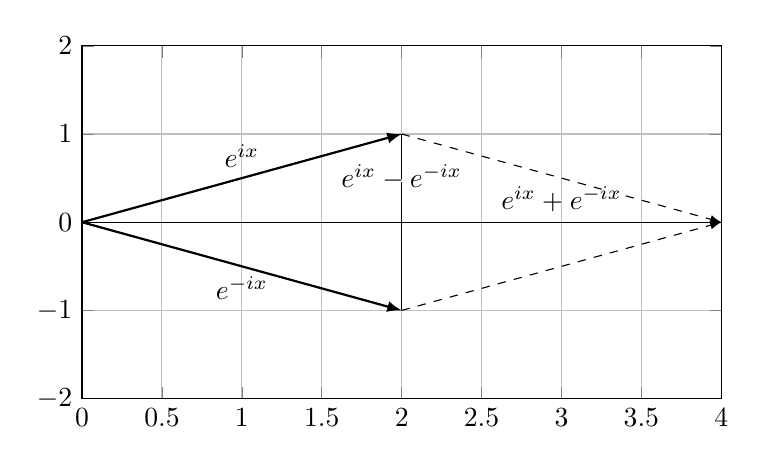
\begin{tikzpicture}
		\begin{axis}[
				xmin=0, xmax=4,
				ymin=-2,ymax=2,
				width=0.8\textwidth, height=0.5\textwidth, grid=major]
			\draw [-latex, thick](0,0)--(2,1) node[midway, above]{$ e^{i x} $};
			\draw [-latex, thick](0,0)--(2,-1)node[midway, below]{$ e^{-i x} $};

			\draw [-latex, dashed](2,1)--(4,0);
			\draw [-latex, dashed](2,-1)--(4,0);

			\draw (0,0)--(4,0) node[pos=0.75, anchor = south]{\contour{white}{$ e^{i x} + e^{-i x}  $}};
			\draw (2,-1)--(2,1)node[pos=0.75]{\contour{white}{$ e^{i x} - e^{-i x}  $}};
		\end{axis}
	\end{tikzpicture}
\end{center}

\subsection{Trigonometria}
\subsubsection*{Formule di duplicazione}
\begin{align*}
	\sin \left(2t\right) & = 2sin\left(t\right) \cos \left(t\right)         \\
	\cos \left(2t\right) & = \cos \left(t\right)^2  - \sin \left(t\right)^2
\end{align*}



\section{Segnali noti e statistiche segnali}
\subsection{Segnali noti}

\subsubsection*{Gradino unitario}
\begin{minipage}[c]{0.48\textwidth}
	\[
		u\left(t\right)   =
		\begin{cases}
			1 & t \ge 0          \\
			0 & \text{ altrove }
		\end{cases}
	\]
\end{minipage}
%
\begin{minipage}[c]{0.48\textwidth}
	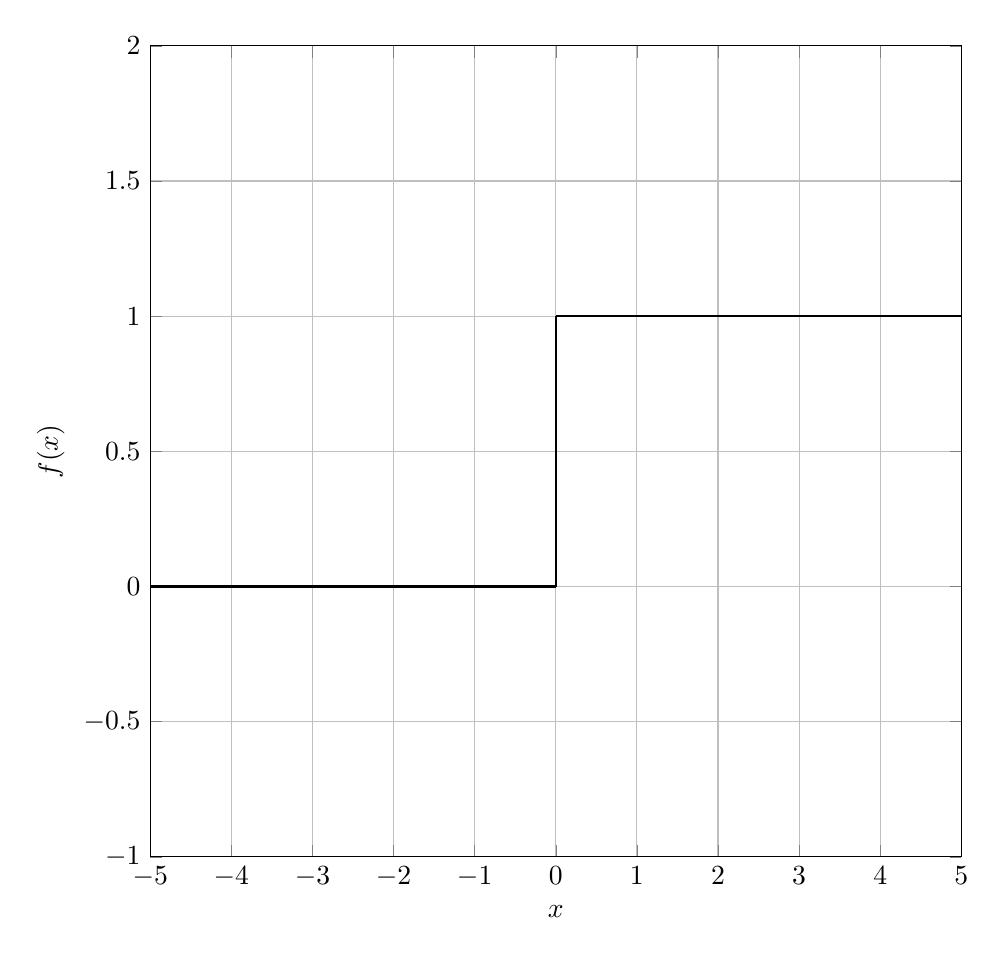
\begin{tikzpicture}
		\begin{axis}[
				xmin=-5, xmax=5,
				ymin=-1,ymax=2,
				width=0.98\textwidth, height=0.98\textwidth, grid=major, samples=200,  ylabel=$f(x)$, xlabel=$x$]
			\addplot[black, thick, domain=-5:0] {0};
			\addplot[black, thick, domain=0:5] {1};
			\draw [thick](0,0)--(0,1);
		\end{axis}
	\end{tikzpicture}
\end{minipage}
\subsubsection*{Funzione segno}
\begin{minipage}[c]{0.48\textwidth}
	\[
		u\left(t\right)   =
		\begin{cases}
			1  & t > 0 \\
			-1 & t < 0
		\end{cases}
	\]
\end{minipage}
%
\begin{minipage}[c]{0.48\textwidth}
	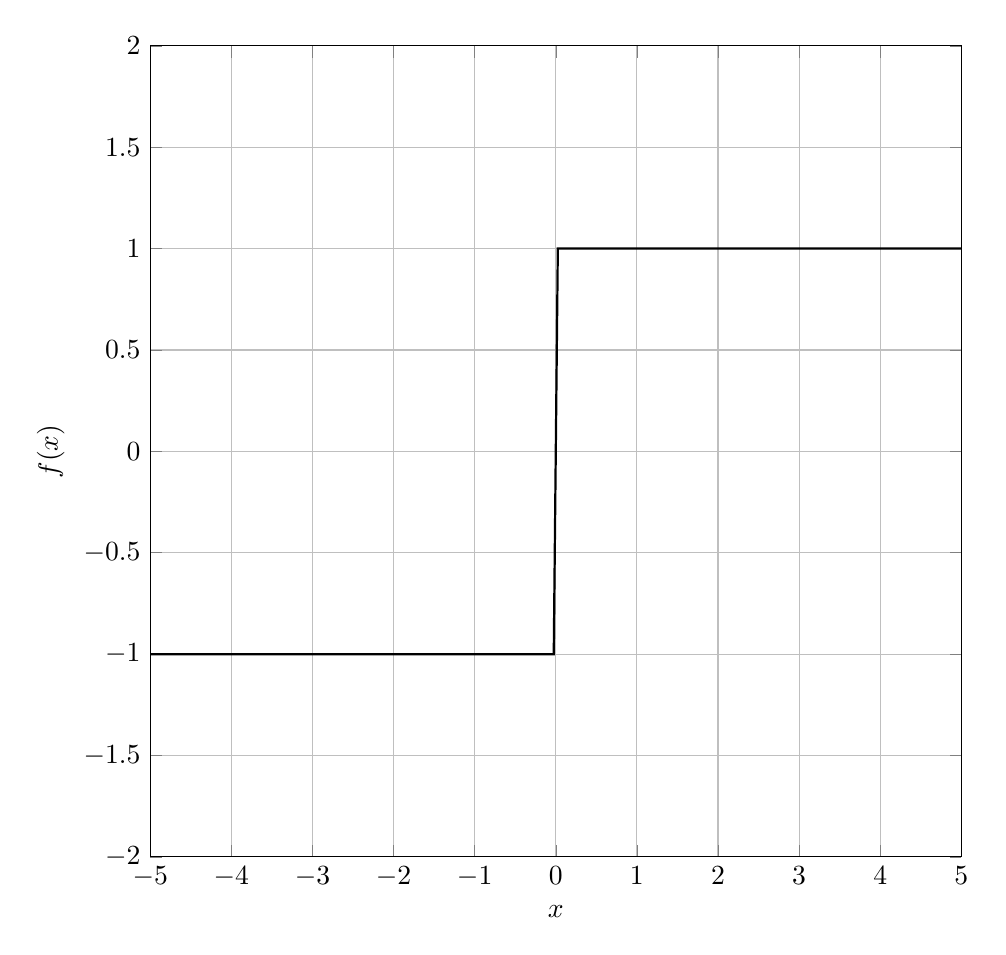
\begin{tikzpicture}
		\begin{axis}[
				xmin=-5, xmax=5,
				ymin=-2,ymax=2,
				width=0.98\textwidth, height=0.98\textwidth, grid=major, samples=200,  ylabel=$f(x)$, xlabel=$x$]
			\addplot[black, thick, domain=-5:5] {sign(x)};
		\end{axis}
	\end{tikzpicture}
\end{minipage}

\subsubsection*{Funzione rettangolo simmetrico}
\begin{minipage}[c]{0.48\textwidth}
	\[
		A \Pi  \left(\frac{t}{T}\right)   =
		\begin{cases}
			A & \left|t\right| \le \frac{T}{2} \\
			0 & \text{ altrove }
		\end{cases}
	\]
\end{minipage}
%
\begin{minipage}[c]{0.48\textwidth}
	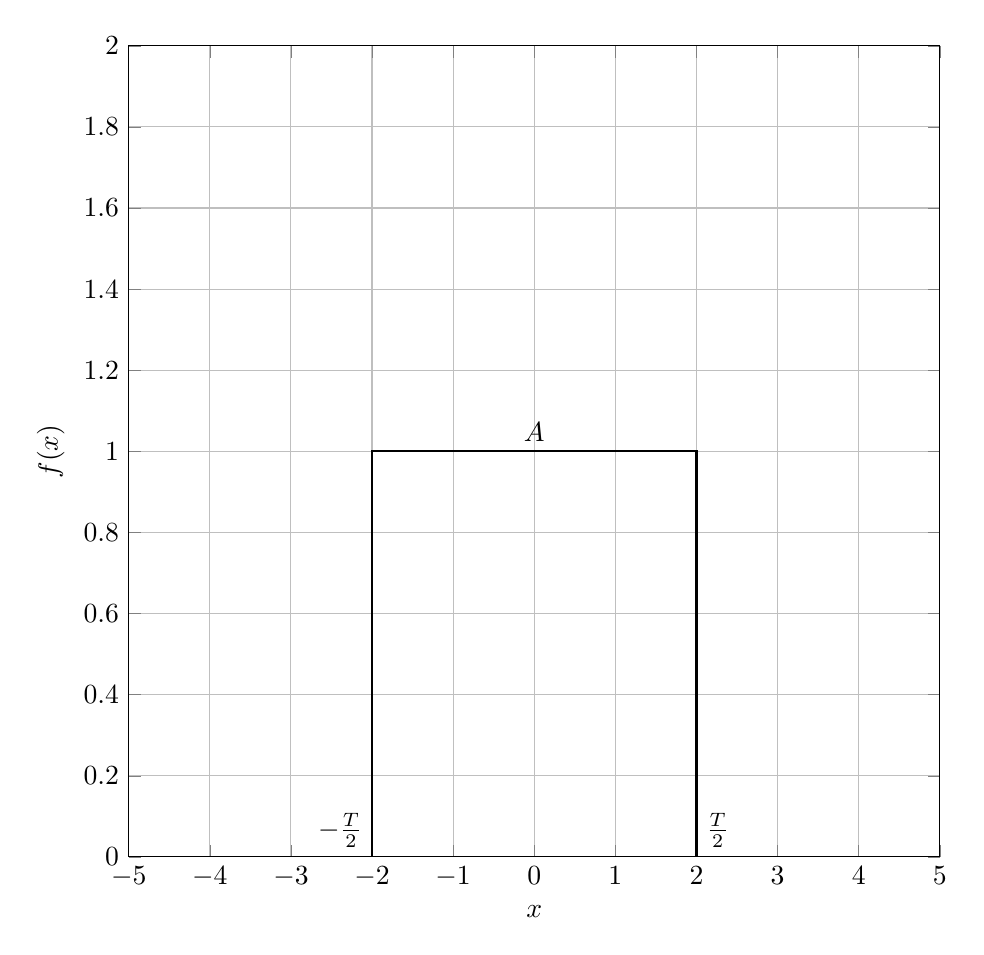
\begin{tikzpicture}
		\begin{axis}[
				xmin=-5, xmax=5,
				ymin=0,ymax=2,
				width=0.98\textwidth, height=0.98\textwidth, grid=major, samples=200,  ylabel=$f(x)$, xlabel=$x$]
			\draw [black, thick](-5,0)--(-2,0)--(-2,1)--(2,1)--(2,0)--(5,0);
			\node ()[anchor = south east] at (-2, 0) {$ -\frac{T}{2} $};
			\node ()[anchor = south west] at (2, 0) {$ \frac{T}{2} $};
			\node ()[anchor = south] at (0, 1) {$ A $};
		\end{axis}
	\end{tikzpicture}
\end{minipage}


\subsubsection*{Funzione triangolo simmetrico}
\begin{minipage}[c]{0.48\textwidth}
	\[
		A \Lambda \left(\frac{t}{T}\right)   =
		\begin{cases}
			\frac{A\left(\frac{T}{2}- \left|t\right|\right)}{T / 2} & \left|t\right| \le \frac{T}{2} \\
			0                                                       & \text{ altrove }
		\end{cases}
	\]
\end{minipage}
%
\begin{minipage}[c]{0.48\textwidth}
	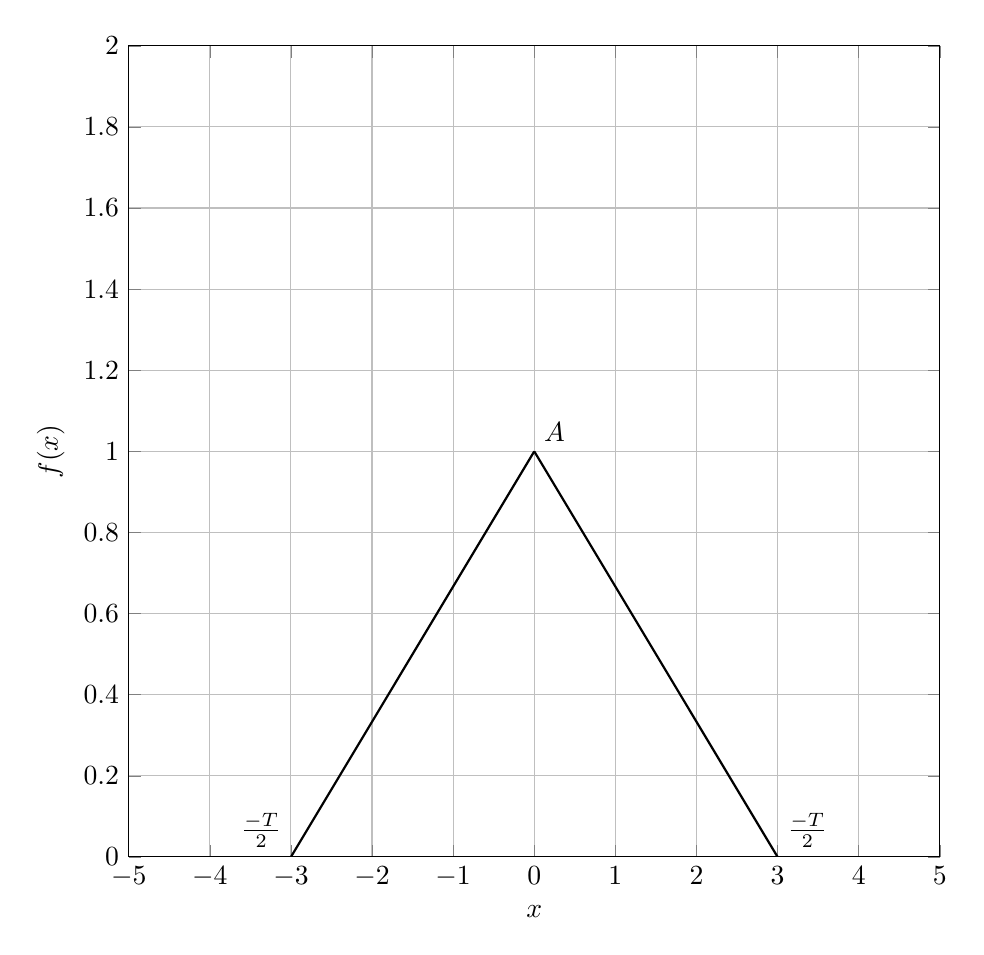
\begin{tikzpicture}
		\begin{axis}[
				xmin=-5, xmax=5,
				ymin=0,ymax=2,
				width=0.98\textwidth, height=0.98\textwidth, grid=major, samples=200,  ylabel=$f(x)$, xlabel=$x$]
			\draw [thick](-3, 0)--(0,1);
			\draw [thick](0,1)--(3, 0);
			\node ()[anchor = south east] at (-3, 0) {$ \frac{-T}{2} $};
			\node ()[anchor = south west] at (3, 0) {$ \frac{-T}{2} $};
			\node ()[anchor = south west] at (0, 1) {$ A $};
		\end{axis}
	\end{tikzpicture}
\end{minipage}

\subsubsection*{Funzione sinc}
\begin{minipage}[c]{0.48\textwidth}
	\[
		\operatorname{sinc}\left(x\right)= \frac{\sin \left(\pi x\right)}{\pi x}
	\]
\end{minipage}
%
\begin{minipage}[c]{0.48\textwidth}
	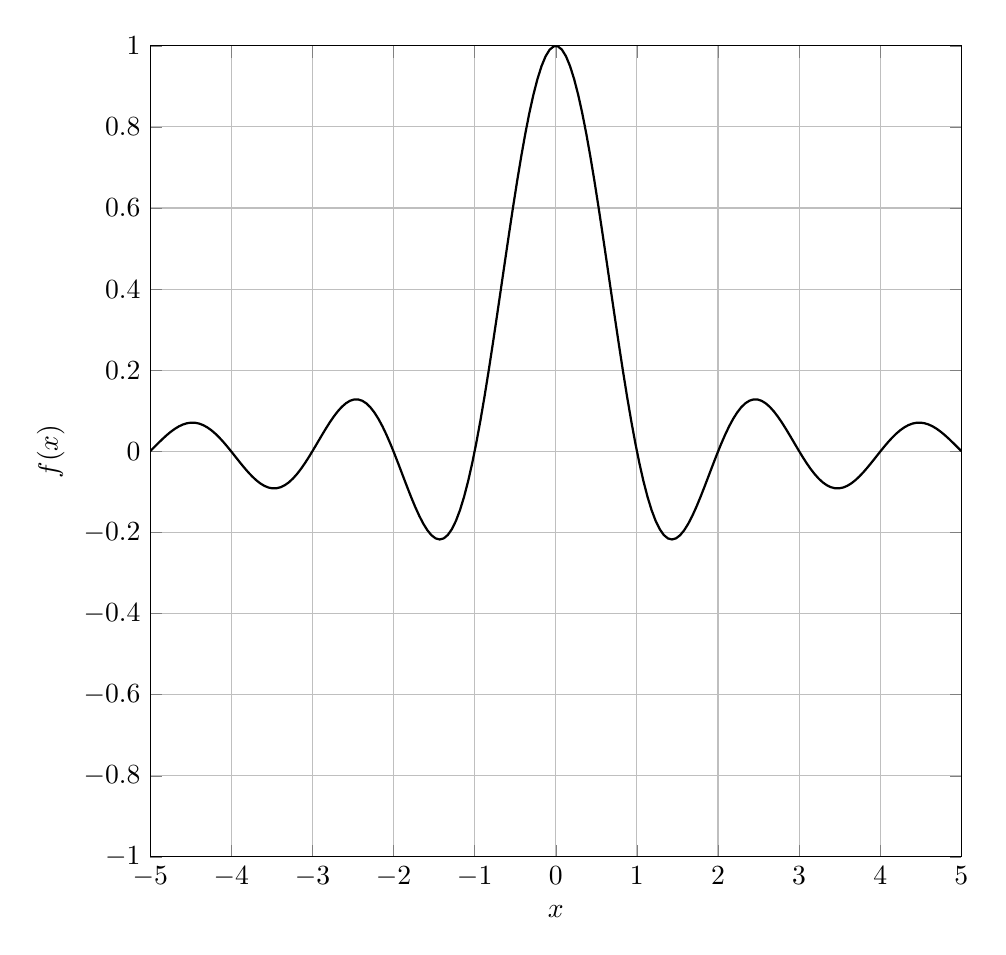
\begin{tikzpicture}
		\begin{axis}[
				xmin=-5, xmax=5,
				ymin=-1,ymax=1,
				width=0.98\textwidth, height=0.98\textwidth, grid=major, samples=200,  ylabel=$f(x)$, xlabel=$x$]
			\addplot[black, thick]{sin(deg(3.14 * x))/(3.14 * x)};
		\end{axis}
	\end{tikzpicture}
\end{minipage}


\subsubsection*{Funzione impulso o delta di Dirac}
\begin{minipage}[c]{0.48\textwidth}
	\[
		\delta \left(t\right) = \lim_{T \to 0} \frac{1}{T} \pi \left(\frac{t}{T}\right) =
		\begin{cases}
			+ \infty & t = 0            \\
			0        & \text{ altrove }
		\end{cases}
	\]

	nota che :
	\[
		\int_{-\infty }^{+ \infty } \delta \left(t\right) \; dt = 1
	\]
	e dunque anche:
	\[
		\int_{-\infty }^{+ \infty } f\left(t\right)\delta \left(t\right) \; dt = f\left(0\right)
	\]
\end{minipage}
%
\begin{minipage}[c]{0.48\textwidth}
	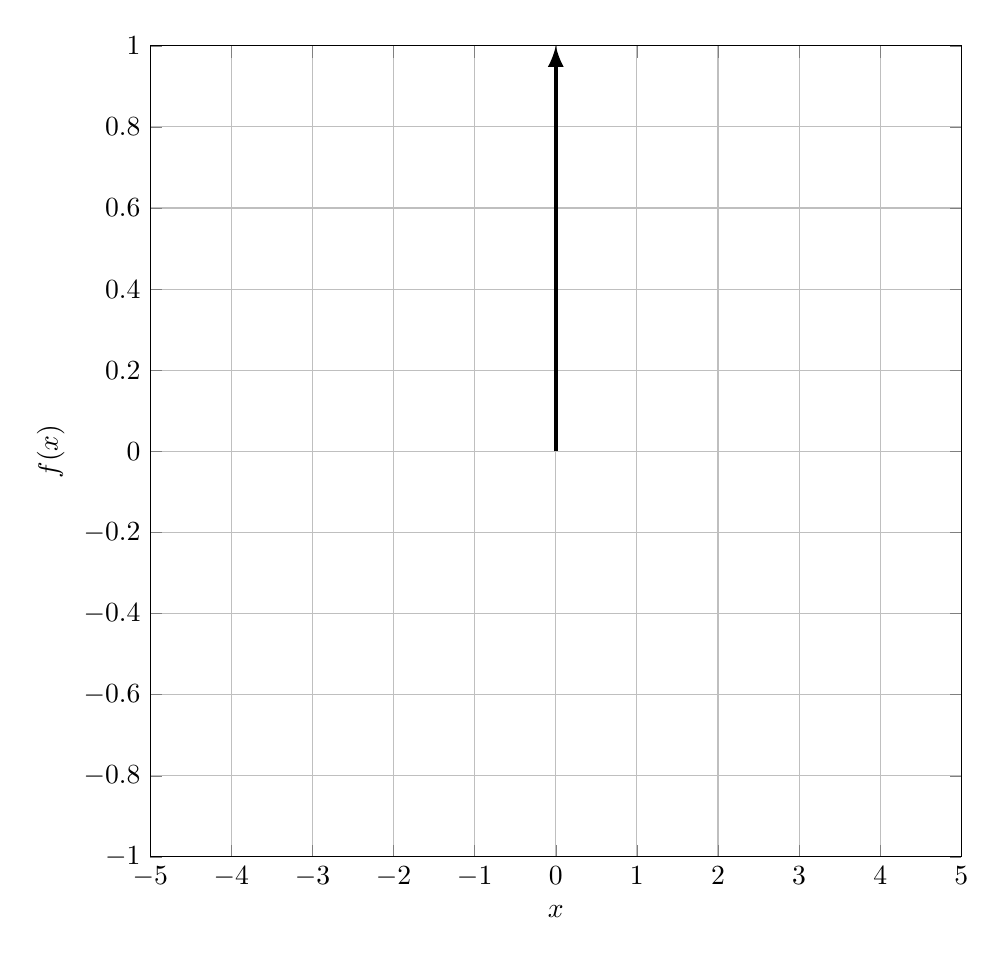
\begin{tikzpicture}
		\begin{axis}[
				xmin=-5, xmax=5,
				ymin=-1,ymax=1,
				width=0.98\textwidth, height=0.98\textwidth, grid=major, samples=200,  ylabel=$f(x)$, xlabel=$x$]
			\draw [-latex][ultra thick](0,0)--(0,1);
		\end{axis}
	\end{tikzpicture}
\end{minipage}
\newpage
\subsection{Statistiche segnali}
\subsubsection*{Valor medio}
\[
	\overline{x} = \left<x\left(t\right)\right> = \lim_{T \to \infty} \frac{1}{T} \int_{\frac{-T}{2}}^{\frac{T}{2}} x\left(t\right) \; dt
\]
\subsubsection*{Valore quadratico medio}
\[
	\overline{x^2 } = \left<x\left(t\right)^2 \right> = \lim_{T \to \infty} \frac{1}{T} \int_{\frac{-T}{2}}^{\frac{T}{2}} x^2 \left(t\right) \; dt
\]

\subsubsection*{Varianza}
\[
	\sigma_x ^2  = \overline{x^2 } - \overline{x}^2 = \lim_{T \to \infty} \frac{1}{T}\int_{\frac{-T}{2}}^{\frac{T}{2}} \left(x\left(t\right)- \overline{x}\right)^2  \; dt
\]
\subsubsection*{Energia}
\[
	E_x = \int_{-\infty }^{\infty } x^2 \left(t\right) \; dt \quad \left[\text{Joule}\right]
\]
\subsubsection*{Potenza}
Uguale a valore quadratico medio:
\[
	\overline{x^2 } = \left<x\left(t\right)^2 \right> = \lim_{T \to \infty} \frac{1}{T} \int_{\frac{-T}{2}}^{\frac{T}{2}} x^2 \left(t\right) \; dt \quad \left[\text{Watt}\right]
\]

Un segnale può essere o di potenza o di energia, non entrambi!

\subsubsection*{Cross correlazione}
Indica intuitivamente quanto due segnali siano simili tra di loro:
\vskip3mm
Se il segnale è di energia:
\[
	R_{xy} = \int_{-\infty }^{\infty } x\left(t\right) y \left(t + \tau \right) \; dt
\]
se invece è di potenza:
\[
	R_{xy} = \lim_{T \to \infty} \frac{1}{T}\int_{-\frac{T}{2} }^{\frac{T}{2} } x\left(t\right) y \left(t + \tau \right) \; dt
\]

se il segnale viene messo in correlazione con se stesso si parla di \textit{autocorrelazione}

\section{Sistemi lti e convoluzione}
\begin{definizione}{Sitema LTI}
	Un sistema è detto LTI se gode di due proprietà:
	\begin{itemize}
		\item Linearità:
		      \[
			      f\left(ax\left(t\right) + bx\left(t\right)\right) = af\left(x\left(t\right)\right) + bf\left(x\left(t\right)\right)
		      \]
		      ossia applicare il sistema sulla somma dei segnali è come sommare l'output dei diversi segnali, una volta passati per il sistema
		\item Tempo invarianza
		      \[
			      f\left(x\left(t\right)\right) = y\left(t\right) \rightarrow f\left(x\left(t- \tau \right)\right) = y\left(t-\tau \right)
		      \]
		      ossia applicare ritardare un segnale non modificherà l'otput del sistema, ad eccezione del ritardo
	\end{itemize}
\end{definizione}

\subsubsection*{Approssimare un segnale con forme d'onda rettangolari}
\[
	X_R\left(t\right) = \sum_{k} x\left(k \Delta T\right) \cdot R\left(t - k  \Delta T\right) \cdot  \Delta T \approx x\left(t\right)
\]
dove $ R\left(t\right) $ è un rettangolo di area unitaria e di ampiezza $ \Delta T $
\subsection{Convoluzione}
Dato un sistema  LTI possiamo calcolare la sua risposta ad una qualsiasi onda se sappaimo la risposta ad un impulso unitario. Data la risposta $ h_R\left(t\right) $ di un sistema alla funzione $ R\left(t\right) $, applicando linearità e tempo invazianza si ottiene:
\[
	x_R\left(t\right) = \sum_{k} x\left(k \Delta T\right) \cdot h_R\left(t - k  \Delta T\right) \cdot  \Delta T
\]
che facendo tendere $ \Delta T $ a 0 diventa:
\[
	\int_{-\infty }^{\infty } x\left(\tau \right) \delta \left(t-\tau \right)  \; d \tau = y\left(t\right)
\]

\begin{definizione}{Convoluzione}
	L'integrale seguente è detto integrale di convoluzione
	\[
		\int_{-\infty }^{\infty } x\left(\tau \right) \delta \left(t-\tau \right)  \; d \tau = y\left(t\right)
	\]
	e rappresenta la risposta di un sistema LTI, calcolabile conoscendo solo la risposta ad un impulso. L'operazione di convoluzione viene rappresentato con un asterisco $ * $
	\[
		x\left(t\right) * h\left(t\right)
	\]
	e si legge $ x\left(t\right) $ convoluito $ y\left(y\right) $
\end{definizione}
Graficamente, effettuare la convouzione significa:
\begin{itemize}
	\item Ribaltare orizzontalmente il segnale
	\item Farlo scorrere orizzontalmente
	\item Di volta in volta integrare
\end{itemize}
\subsubsection*{Properietà convoluzione}
\begin{itemize}
	\item La convoluzione restituisce una funzione che ha durata $ \ge  $ della funzione di partenza, omeglio $ =  $ alla somma delle durate delle due funzioni
	\item Proprietà commutativa
	      \[
		      x(t) * y(t)=y(t) * x(t) \\
	      \]
	\item Proprietà associativa
	      \[
		      x(t) * y(t) * \mathrm{z}(\mathrm{t})=x(\mathrm{t}) *[y(t) * z(t)] \\
	      \]
	\item Properità distributiva
	      \[
		      x(t) *[y(t)+z(t)]=x(t) * y(t)+x(t) * z(t)
	      \]
	\item Linearità
	      \[
	      \]
\end{itemize}
\subsubsection*{Convoluzioni notevoli}
\begin{enumerate}
	\item Rettangoli simmetrici di pari durata: triangolo simmetrico di ampiezza  $ 2T $ e area $ A_1 \cdot  A_2 \cdot T $
	      \[
		      A \Pi \left(\frac{t}{T}\right) * A_2 \Pi \left(\frac{t}{T}\right) = A_1A_2T \Lambda \left(\frac{t}{2T}\right)
	      \]
	\item Rettangoli dimmetrici di durata diversa: assumento $ T_1 \ge T_2 $ ottengo trapezio con
	      \begin{itemize}
		      \item $ B = T_1  + T_2 $
		      \item  $ b = T_2 - T_1 $
		      \item  $ h = A_1 \cdot A_2 \cdot  T_1 $
	      \end{itemize}
	\item Rettangoli non simmetrici: come rettangoli simmetrici ma centrati nel mezzo del rettangolo con lunghezza maggiore
	\item Gaussiana: date
	      \[
		      x_1(t)=\frac{1}{\sqrt{2 \pi \sigma_1^2}} e^{-\frac{\left(t-\mu_1\right)^2}{2 \sigma_1^2}} ; x_2(t)=\frac{1}{\sqrt{2 \pi \sigma_2^2}} e^{-\frac{\left(t-\mu_2\right)^2}{2 \sigma_2^2}}
	      \]
	      allora la convoluzione vale
	      \[
		      y(t)=x_1(t) * x_2(t)=\frac{1}{\sqrt{2 \pi\left(\sigma_1^2+\sigma_2^2\right)}} e^{-\frac{\left[t-\left(\mu_1+\mu_2\right)\right]^2}{2\left(\sigma_1^2+\sigma_2^2\right)}}
	      \]
\end{enumerate}
\section{Serie e trasformata di Fourier}

\begin{definizione}{Serie di Fourier}
	La serie di fourirer è cosi definita:
	\[
		x\left(t\right) = a_0 + \sum_{k} \cos \left(2 \pi k f_0 t + \omega_k  \right)
	\]
	passando alla notazione con i numeri complessi, si ottiene:
	\begin{align*}
		 & x(t)=\sum_{n=-\infty}^{+\infty} X_n e^{j 2 \pi n f_0 t} &  &
		 & X_n=
		\begin{cases}
			\frac{a_n}{2} e^{j \vartheta_n}       & n>0 \\
			\frac{a_{-n}}{2} e^{j \vartheta_{-n}} & n<0 \\
			a_0                                   & n=0
		\end{cases}
	\end{align*}
	i coefficienti della serie sono calcolati come segue:
	\[
		X_n=\frac{1}{T_0} \int_{-T_0 / 2}^{T_0 / 2} x(t) e^{-j 2 \pi n f_0 t} d t
	\]
\end{definizione}

Proprietà serie di fourier:
\begin{enumerate}
	\item Simmetria Hermitiana:
	      \[
		      X_n=-X_{-n}^* \Leftrightarrow\left\{\begin{array}{l}
			      \left|X_n\right|=\left|X_{-n}\right| \\
			      \arg \left(X_n\right)=-\arg \left(X_{-n}\right)
		      \end{array}\right.
	      \]

	\item Linearità: dati $x(t)$ e $y(t)$ periodici, avremo
	      \[
		      z(t)=\alpha x(t)+\beta y(t) \Rightarrow Z_k=\alpha X_k+\beta Y_k
	      \]
	\item Simmetrie del segnale:
	      \begin{enumerate}
		      \item Periodico \textit{pari} $ \rightarrow $ coefficienti $X_n$ reali $ \rightarrow  $ soli coseni
		            \[
			            X_k=\frac{2}{T_0} \int_0^{T_0 / 2} x(t) \cos \left(2 \pi k f_0 t\right) d t
		            \]
		      \item  Periodico \textit{dispari} $ \rightarrow $ coefficienti $X_n$ immaginari $ \rightarrow  $ soli seni
		            \[
			            X_k=-\frac{2 j}{T_0} \int_0^{T_0 / 2} x(t) \sin \left(2 \pi k f_0 t\right) d t
		            \]
		      \item Segnale \textit{alternato} $ \rightarrow  $ ho solo armoniche \underline{dispari}
	      \end{enumerate}
	      NB. date le simmetrie, posso calcolare l'integrale su metà periodo
\end{enumerate}

\begin{definizione}{Trasformata di Fourier}
	La traformata di Fourier può essere intesa come il limite per $ T_0 \to  \infty  $ della serie di Fourier
	\[
		w\left(t\right) = \int_{-\infty }^{\infty } X\left(f\right) e ^{ j 2 \pi  f t}df \; dx
	\]
	dove i coefficienti $ X\left(f\right) $ sono:
	\[
		X\left(f\right) = \int_{-\infty }^{\infty } w\left(t\right)e^{-j_2 \pi  ft} \; dx
	\]
\end{definizione}
La prima si ottiene facendo il limite per $ x \to  \infty  $ della serie di Fourier:
\begin{align*}
	\sum_{k = -\infty}^{\infty} X_ke^{j 2 \pi k f_0 t } & =\sum_{k = -\infty}^{\infty} X_k \frac{T_0}{T_0} e^{j 2 \pi k f_0 t }    \\
	                                                    & =\sum_{k = -\infty}^{\infty} X_k T_0 e^{j 2 \pi k f_0 t } f_0            \\
	                                                    & =\sum_{k = -\infty}^{\infty} X\left(kf_0\right) e^{j 2 \pi k f_0 t } f_0 \\
\end{align*}
passando al limite per $ T_0 \to  \infty  $ e dunque $ f_0 \to 0 $, $ kf_0 $ tende a una variabile continua $ f $ e $ f_0 $ a un infinitesimo $ df $:
\begin{align*}
	\lim_{T_0 \to \infty} \sum_{k = -\infty}^{\infty} X\left(kf_0\right) e^{j 2 \pi k f_0 t } f_0 & = \lim_{T_0 \to \infty} \sum_{k = -\infty}^{\infty} X\left(f\right) e^{j 2 \pi f t } df \\
\end{align*}
dunque:
\[
	w\left(t\right) = \int_{-\infty }^{\infty } X\left(f\right) e^{j 2 \pi f t} df \; dx
\]
Applicando lo stesso limite a $ X\left(f\right) $, ottengo come calcolarmi i coefficienti:
\begin{align*}
	X\left(f\right) = \lim_{f_0 \to 0} X\left(kf_0\right)= \lim_{t_0 \to \infty} \int_{-\frac{T_0}{2}}^{\frac{T_0}{2}} w\left(t\right)e^{-2 \pi  j k f_0 t} \; dt
\end{align*}
dunque
\[
	X\left(f\right) = \int_{-\infty }^{\infty } w\left(t\right) e^{-j 2 \pi f t} dt
\]
\subsubsection*{Proprietà trasformata di Fourier}
\begin{enumerate}
	\item Simmetria Hermitiana se $ x\left(t\right) $ funzione reale
	\item Linearità
	\item Simmetrie segnale nel tempo
	      \begin{align*}
		      x(t) \in \mathbb{R} \text { pari }    & \Rightarrow X(f)=2 \int_0^{+\infty} x(t) \cos (2 \pi f t) d t    \\
		      x(t) \in \mathbb{R} \text { dispari } & \Rightarrow X(f)=-2 j \int_0^{+\infty} x(t) \sin (2 \pi f t) d t
	      \end{align*}
	\item Fattore di scala:
	      \[
		      x\left(t\right) \Leftrightarrow X\left(f\right) \Rightarrow x\left(\alpha t\right) \Leftrightarrow \frac{1}{\alpha }X \left(\frac{f}{\alpha} \right)
	      \]
	      ossia, se il segnale viene compresso, allora le sue frequenze aumentano (immagina di velocizzare audio)
	\item Fattore di ritardo:
	      \[
		      x\left(t - \Delta T \right) \rightarrow X\left(f\right)e^{-j2 \pi f \Delta T }
	      \]
	\item Dualità:
	      \[
		      x\left(t\right) \rightarrow y\left(f\right) \Leftrightarrow y\left(t\right) \rightarrow  x\left(-f\right)
	      \]
	\item Derivata:
	      \[
		      \mathfrak{F}\left\{ \frac{d}{dt} \left[x\left(t\right)\right]\right\} = j 2 \pi f \cdot X\left(f\right)
	      \]
	\item Integrale
	      \[
		      \mathfrak{F}\left\{\int_{-\infty }^{t} x\left(\varepsilon \right) \; d\varepsilon \right\} = \frac{X\left(f\right)}{j 2 \pi  f} + \frac{X\left(0\right)}{2} \delta \left(f\right)
	      \]
	\item Convoluzione
	      \[
		      \mathfrak{F} \left\{x\left(t\right)* y\left(t\right)\right\} = \mathfrak{F}\left(x\left(t\right)\right) \cdot \mathfrak{F}\left(y\left(t\right)\right)
	      \]
	\item Prodotto
	      \[
		      \mathfrak{F} \left\{x_1\left(t\right) \cdot  x_2\left(t\right)\right\} = \mathfrak{F} \left\{x_1\left(t\right)\right\} * \mathfrak{F} \left\{x_2\left(t\right)\right\}
	      \]
\end{enumerate}
\subsection{Trasformate notevoli}
\begin{enumerate}
	\item Rettangolo:
	      \begin{align*}
		      V_0 \Pi  \left(\frac{t}{T}\right) \rightarrow  V_0 T \operatorname{sinc}\left(f T\right)
	      \end{align*}
	\item Sinc function:
	      \begin{align*}
		      V_0 \operatorname{sinc} \left(t W\right) = V_0
	      \end{align*}
	\item Costante
	      \[
		      \mathfrak{F} \left\{V_0\right\}= V_0 \delta  \left(f\right)
	      \]
	\item Esponenziale
	      \[
		      \mathfrak{F} \left\{e^{-\alpha t}\right\} = \frac{1}{\alpha  + j 2 \pi  f}
	      \]
	\item Sinusoidi
	      \begin{align*}
		      \mathfrak{F}\left\{\cos \left(2 \pi f_0 t\right)\right\}  & = \frac{1}{2}\left[\delta\left(f+f_0\right)+\delta\left(f-f_0\right)\right] \\
		      \mathfrak{F}\left\{\sin  \left(2 \pi f_0 t\right)\right\} & = \frac{1}{2}\left[\delta\left(f+f_0\right)-\delta\left(f-f_0\right)\right] \\
	      \end{align*}
	\item Impulso
	      \[
		      \mathfrak{F}\left\{\delta \left(t- t_0\right)\right\} = 1 \cdot e ^{ -j 2 \pi  f t_0}
	      \]
	\item Treno di impulsi
	      \begin{align*}
		      \mathfrak{F}\left\{\sum_{n= -\infty }^{\infty} \delta \left(t - nT\right)\right\} = \frac{1}{T} \sum_{n= -\infty}^{\infty} \sigma \left(f - \frac{n}{T}\right)
	      \end{align*}
\end{enumerate}

\subsection{Energia e banda}
\begin{teorema}{Parseval}
	Dato un segnale periodico, la sua potenza è uguale a:
	\[
		P_x = \sum_{k=-\infty }^{\infty} \left|X_n\right|^2
	\]
\end{teorema}
Questo teorema può essere esteso segnali non periodici
\begin{teorema}{Rayleigh}
	Dato un segnale aperiodico, la sua energia è uguale a:
	\[
		E_x = \int_{-\infty }^{\infty } \left|x\left(t\right)\right|^2  \; dt = \int_{-\infty }^{\infty } \left|X\left(f\right)\right|^2 \; df
	\]
\end{teorema}
\begin{definizione}{Larghezza di banda}
	La larghezza di banda è l'intervallo di frequenze per le quali lo spettro del segnale assume valori non nulli. Per segnali con spettro infinito, si può imporre la larghezza di banda come l'intervalli in cui p contenuto l'$ x $ \% della energia del segnale:
	\[
		B: \int_{-B}^{B} \left|X\left(f\right)\right|^2  \; df = 0.99Ex
	\]
\end{definizione}

per dualità ho che $ F\left(x\left(t\right)\right) = Y\left(f\right) \rightarrow F\left(Y\left(t\right)\right)= x\left(-f\right) $. Dunque è anche vero che
\newpage
\section{Distorsione ed equalizzazione}
\begin{definizione}{Condizione di non distorsione}
	Un sistema è non distorcente se la sua risposta in frequenza è piatta e la sua risposta in fase è lineare (una retta)

	\begin{minipage}[t]{0.48\textwidth}
		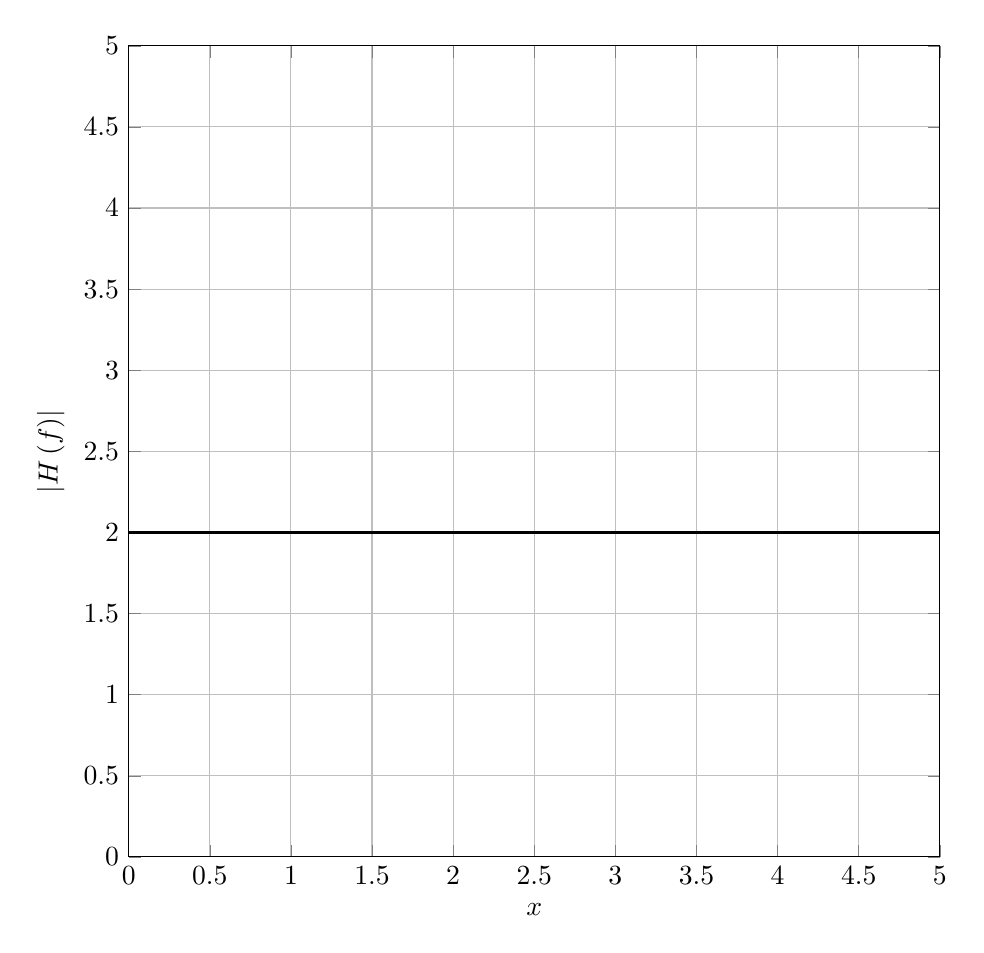
\begin{tikzpicture}
			\begin{axis}[
					xmin=0, xmax=5,
					ymin=0,ymax=5,
					restrict y to domain = 0:5, domain=0:5, width=0.98\textwidth, height=0.98\textwidth, grid=major, samples=200,  ylabel=$\left|H\left(f\right)\right|$, xlabel=$x$]
				\addplot[black, thick] {2};
			\end{axis}
		\end{tikzpicture}
	\end{minipage}
	%
	\begin{minipage}[t]{0.48\textwidth}
		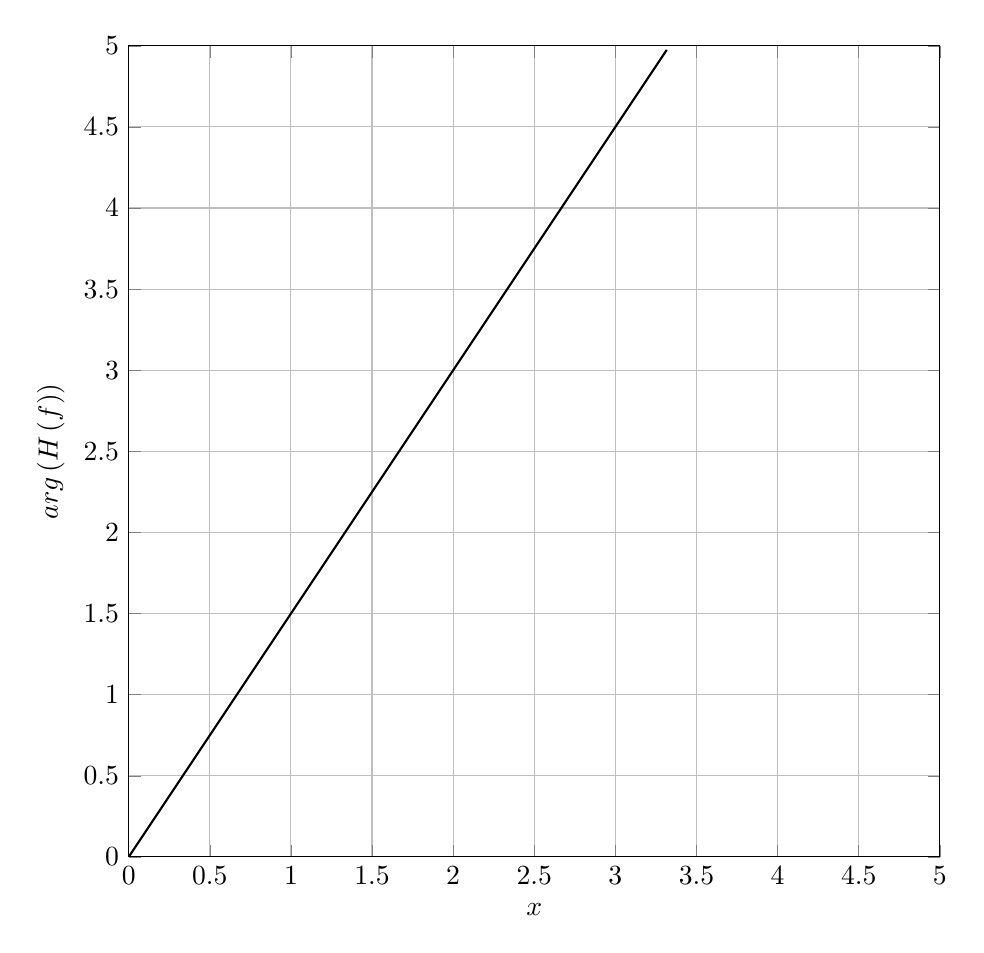
\begin{tikzpicture}
			\begin{axis}[
					xmin=0, xmax=5,
					ymin=0,ymax=5,
					restrict y to domain = 0:5, domain=0:5, width=0.98\textwidth, height=0.98\textwidth, grid=major, samples=200,  ylabel=$\operatorname{arg}\left(H\left(f\right)\right)$, xlabel=$x$]
				\addplot[black, thick] {1.5*x};
			\end{axis}
		\end{tikzpicture}
	\end{minipage}
\end{definizione}
\begin{definizione}{Ritardo di gruppo}
	Il ritardo di gruppo(temporale) è dato dallo sfasamento di fase di un segnale:
	\[
		\tau_g\left(f\right) = -\frac{d \phi\left(f\right) }{df}
	\]
\end{definizione}
Se il sistema è LTI, allora si può compensare la distorsione applicando un'equalizzazione tale per cui:
\[
	H_{\text{ tot }} = H\left(f\right) \cdot  H_{\text{ eq }} = k e ^{-j 2 \pi f t_0}
\]
\subsection{Distorsione non lineare}
Se il sistema non è LTI, allora
\begin{itemize}
	\item Spettro si deforma e si \underline{allarga}
	\item Posso calcolare \underline{distorsione di seconda armonica}
	      \[
		      \text{ distorsione di seconda armonica } = \left|\frac{\beta }{\alpha }\right| \cdot 100
	      \]
	\item Posso fare companding per evitare distorsione:
	      \begin{center}
		      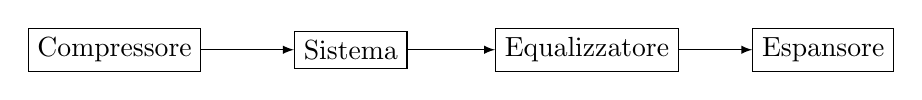
\begin{tikzpicture}
			      \node (a) [draw] {Compressore};
			      \node (b) [draw, right of=a, xshift=2cm] {Sistema};
			      \node (c) [draw, right of=b, xshift=2cm] {Equalizzatore};
			      \node (d) [draw, right of=c, xshift=2cm] {Espansore};
			      \draw [-latex](a)--(b);
			      \draw [-latex](b)--(c);
			      \draw [-latex](c)--(d);
		      \end{tikzpicture}
	      \end{center}

\end{itemize}
\section{Conversione AD/DA}
\subsection{Campionamento nel tempo - versione teorica}
Matematicamente posso rappresentare il campionamento nel tempo come:
\[
	x_c\left(t\right) = \sum_{n= -\infty }^{\infty} x\left(n T_c\right) \delta \left(t - n T_c\right)
\]
Passando al dominio della frequenza ottengo
\[
	X_c\left(f\right) = X\left(f\right) * \frac{1}{T_c} \sum_{n = -\infty }^{\infty} \delta \left(f - kf_c\right)
\]
Nota dunque come si ottenga il preciso spettro di $ x\left(t\right) $ ripetuto nel tempo.
Per risalire al segnale originario posso sfruttare un low cut, finestrando la prima iterazione del suo spettro:
\vskip3mm
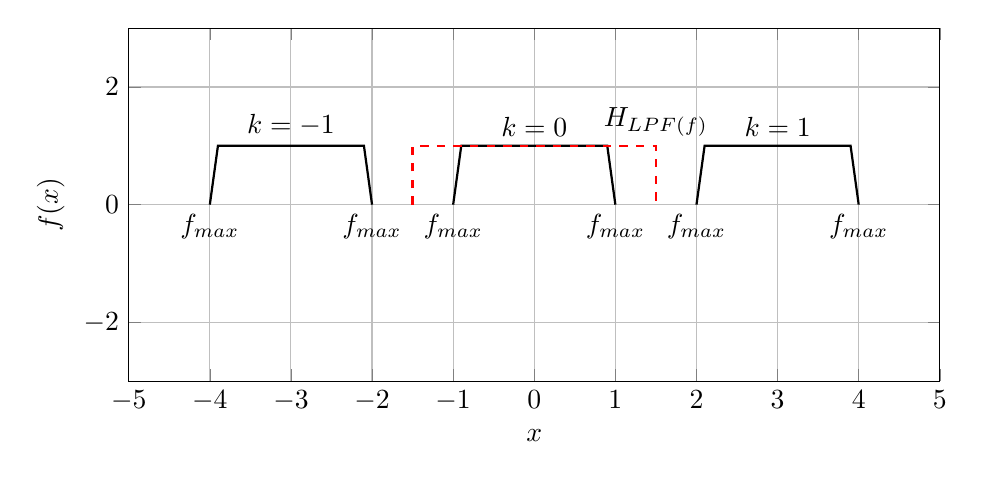
\begin{tikzpicture}

	\begin{axis}[
			xmin=-5, xmax=5,
			ymin=-3,ymax=3,
			restrict y to domain = -3:3, domain=-5:5, width=0.98\textwidth, height=0.5\textwidth, grid=major, samples=200,  ylabel=$f(x)$, xlabel=$x$]
		\coordinate (center) at (0,0);
		\draw [black, thick](-1, 0)--(-0.9, 1) -- (0.9, 1) -- (1, 0);
		\draw [black, thick](-1+3, 0)--(-0.9+3, 1) -- (0.9+3, 1) -- (1+3, 0);
		\draw [black, thick](-1-3, 0)--(-0.9-3, 1) -- (0.9-3, 1) -- (1-3, 0);
		\node [anchor = south]at (-3, 1)  {$ k = -1 $};
		\node [anchor = south]at (0, 1)  {$ k = 0 $};
		\node [anchor = south]at (3, 1)  {$ k = 1 $};

		\node [anchor = north]at (-2, 0)  {$f_{\text{max}}$};
		\node [anchor = north]at (-4, 0)  {$f_{\text{max}}$};
		\node [anchor = north]at (-1, 0)  {$f_{\text{max}}$};
		\node [anchor = north]at (1, 0)  {$f_{\text{max}}$};
		\node [anchor = north]at (2, 0)  {$f_{\text{max}}$};
		\node [anchor = north]at (4, 0)  {$f_{\text{max}}$};

		\draw [dashed, red, thick](-1.5,0)--(-1.5,1)--(1.5,1)--(1.5,0);
		\node [anchor = south]at (1.5, 1){$ H_{\text{LPF}\left(f\right)} $};
	\end{axis}

\end{tikzpicture}
\vskip3mm
Questo ricostruisce perfettamente il segnale, ma solo nel caso in cui $ f_c \ge f_{\text{max}} $. Da qui la regola di Nyquist:
\begin{definizione}{Regola di Nyquist}
	Per campionare un segnale senza perdita di informazione (aliasing) deve valere che.
	\[
		f_c \ge 2 f_{\text{max}} \quad  \text{o equivalentemente} \quad T_c < \frac{1}{2} T_{\text{max}}
	\]
\end{definizione}

Per ricostuire il campione mi basta quindi applicare un passa-basso:
\begin{align*}
	x'\left(t\right) & = \sum_{k=-\infty }^{\infty} x\left(nT_c\right)\delta \left(t - nT_c\right) * \operatorname{sinc} \left(\frac{t}{T_c}\right) \\
	                 & = \sum_{k=-\infty }^{\infty} x\left(nT_c\right) \operatorname{sinc} \left(\frac{t - nT_c}{T_c}\right)
\end{align*}

\subsection{Campionamento nel tempo - sample and hold}
Nella pratica viene usata una tecnica diversa.
\begin{center}
	\includegraphics[width = 0.7\textwidth]{Images/Sample and hold.png }
\end{center}
\begin{itemize}
	\item Siccome $ h_H\left(t\right) $ in frequenza diventa una sinc, le frequenze verranno attenuate. Questo è compensabile tramite un'equalizzazione
\end{itemize}
\begin{figure}[H]
	\begin{center}
		\includegraphics[width = 0.7\textwidth]{Images/Sample and hold 2.png}
	\end{center}
	\caption{Si noti come la curva blu, ossia il filtro di trattenimento attenui le frequenze alte}
\end{figure}
\begin{figure}[H]
	\begin{center}
		\includegraphics[width = 0.7\textwidth]{Images/Sample and hold 3.png}
	\end{center}
	\caption{Filtro di equalizzazione per contrastare effetto del filtro di trattenimento}
\end{figure}
\subsection{Quantizzazione}
Posso stimare la potenza dell'"errore" di quantizzazione assumendo che questo sia distribuito in maniera omogenea:
\begin{figure}[H]
	\begin{center}
		\includegraphics[width = 0.4\textwidth]{Images/Quantizzazione 1.png}
	\end{center}
	\caption{Distribuzione di probabilità di errore di quantizzazione}
\end{figure}
La potenza coincide con il valore quadratico medio, che a sua volta
coincide con la varianza, dato che la distribuzione appena vista ha
chiaramente valor medio nullo
\[
	E\left\{\varepsilon_q^2\right\}=\sigma_q^2=\int_{-\frac{\Delta}{2}}^{\frac{\Delta}{2}} \varepsilon^2 f_{\varepsilon_q}(\varepsilon) d \varepsilon=\frac{1}{\Delta} \int_{-\frac{\Delta}{2}}^{\frac{\Delta}{2}} \varepsilon^2 d \varepsilon=\left.\frac{1}{\Delta} \frac{\varepsilon^3}{3}\right|_{-\frac{\Delta}{2}} ^{\frac{\Delta}{2}}=\frac{\Delta^2}{12}
\]
Per stimare la qualità del segnale di utilizza il rapporto fra potenza di rumore e posenza del segnale:
\begin{definizione}{Rapporto segnale rumore}
	Il rapporto segnale rumore è così definito:
	\[
		\text{SNR} = 10 \log _{10} \left(\frac{S_x}{S_n}\right) \left[\text{db}\right]
	\]
	Ogni bit in più usato per rappresentare la quantizzazione corrisponse a circa \underline{6 db} in i più nel $ SNR $
\end{definizione}
Salvare segnale è costoso in termini di spazio. Ad esempio per salvare un segnale con $ f_{\text{max}} = 10 kh $ con qualità di almeno 30 db servono:
\[
	r_b \ge \underbracket[0.1ex]{2 \cdot  10^{4}}_{\text{Nyquist}} \cdot \underbracket[0.1ex]{\frac{30}{6}}_{\text{db ogni bit in più}} = 10^{5} \left[\frac{\text{bits}}{\text{sec}}\right]
\]
\subsection{Modulazione predittiva}
Tecniche per salvare bit
\subsubsection*{Modulazione delta}
Scelgo costante $ \Delta  $ a priori e per ogni campione esprimo il suo valore in funzione del precedente $ \pm \Delta  $.
\[
	x_i = n_{i-1} \pm \Delta
\]
Problemi:
\begin{itemize}
	\item Staircase
	\item Slope overload
	\item Quantization noise
\end{itemize}
\subsubsection*{Modulazione DPCM}
Crea una stima del valore del campione presente utilizzando i campioni passati e salva l'errore rispetto alla stima in un dato numero di bits, ad esempio:
\[
	\hat{x_i} = a_1 \tilde{x_{i-1}} + a_2 \tilde{x_{i-2}} + \ldots + a_N \tilde{x_{i-N}}
\]

\section{Segnali discreti: basi}

\begin{enumerate}
	\item Simmetria:
	      \begin{itemize}
		      \item Pari:
		            \[
			            x(t) = x(-t) \quad \forall t \Rightarrow  x[n] = x[-n] \quad \forall n
		            \]
		      \item Dispari:
		            \[
			            x(t) = -x(-t) \quad \forall t \Rightarrow  x[n] = -x[-n] \quad \forall n
		            \]
	      \end{itemize}

	\item Guadagno:
	      \begin{itemize}
		      \item Positivo:
		            \[
			            \alpha x(t) : \alpha > 1 \Rightarrow \alpha x[n] : \alpha > 1
		            \]
		      \item Negativo:
		            \[
			            \alpha x(t) : \alpha < 1 \Rightarrow \alpha x[n] : \alpha < 1
		            \]
	      \end{itemize}

	\item Ritardo:
	      \[
		      x(t - \Delta T) \Rightarrow x[n - k]
	      \]

	\item Integrazione discreta:
	      \[
		      y[n] = \sum_{k=-\infty}^{n} x[k]
	      \]

	\item Derivazione discreta:
	      \[
		      y[n] = \frac{1}{T_c} (x[n] - x[n-1])
	      \]
	      $ T_c = 1$ se non conosciuto

	\item Convoluzione discreta:
	      \[
		      y[n] = x[n] * h[n] = \sum_{k=-\infty}^{\infty} x[k] h[n-k]
	      \]

\end{enumerate}
\subsection{Statistiche segnali discreti}
\begin{enumerate}

	\item Valor medio:
	      \[
		      \bar{x} = \lim_{T \to \infty} \frac{1}{T} \int_{-T/2}^{T/2} x(t) \, dt \implies \bar{x} = \lim_{K \to \infty} \frac{1}{K} \sum_{k=1}^{K} x[k]
	      \]

	\item Varianza:
	      \[
		      \sigma_x^2 = \lim_{T \to \infty} \frac{1}{T} \int_{-T/2}^{T/2} \left(x(t) - \bar{x}\right)^2 \, dt \implies \sigma_x^2 = \lim_{K \to \infty} \frac{1}{K} \sum_{k=1}^{K} \left(x[k] - \bar{x}\right)^2
	      \]

	\item Energia:
	      \[
		      E_x = \int_{-\infty}^{\infty} |x(t)|^2 \, dt \implies E_x = \sum_{k=-\infty}^{\infty} |x[k]|^2
	      \]

	\item Potenza media:
	      \[
		      P_x = \lim_{T \to \infty} \frac{1}{T} \int_{-T/2}^{T/2} |x(t)|^2 \, dt \implies P_x = \lim_{K \to \infty} \frac{1}{K} \sum_{k=1}^{K} |x[k]|^2
	      \]

	\item Cross-correlazione:
	      \[
		      R_{xy}[k] = \sum_{n=-\infty}^{\infty} x[n] y[n+k]
	      \]

	\item Autocorrelazione:
	      \[
		      R_x[k] = \sum_{n=-\infty}^{\infty} x[n] x[n+k]
	      \]

	\item Istogramma:
	      \begin{itemize}

		      \item Creazione \[
			            h(l) = \frac{1}{N} \sum_{n=1}^{N} \delta(x[n] - v_l), \quad l = 1, \dots, L
		            \]
		      \item Valor medio
		            \[
			            \bar{x}=\sum_{l=1}^L v[l] \cdot h[l]
		            \]
		      \item Varianza
		            \[
			            \sigma_x^2=\sum_{l=1}^L(v[l]-\bar{x})^2 \cdot h[l]
		            \]
	      \end{itemize}

\end{enumerate}

\subsection{Filtri}
\begin{enumerate}
	\item Passa basso (LPF)
	      \begin{enumerate}
		      \item Media mobile (filtro passa-basso FIR):
		            \[
			            h[k] = \frac{1}{K} \cdot [1, 1, \dots, 1]
		            \]

		      \item Gaussiana discreta (kernel di convoluzione):
		            \[
			            h[k] = \frac{1}{\lambda} e^{-\frac{k^2}{2\sigma^2}}, \quad k \in \left[-\frac{K}{2}, \frac{K}{2}\right]
		            \]
		            dove $\lambda  = \sum_{k} e^{- \frac{k^2 }{2 \sigma  ^2 }}$ e $ \sigma ^2  $ è la varianza.
	      \end{enumerate}
	\item Passa alto (HPF)
	      Si possono ottenere per differenza:
	      \[
		      h_{\text{HPF}} = \delta \left[k\right] - h_{\text{LPF}}\left[k\right]
	      \]
	\item Derivativi e integrativi:
	      \begin{enumerate}
		      \item Filtro gradiente (derivata prima):
		            \[
			            h[k] = [-1, 1]
		            \]

		      \item Filtro Laplaciano (derivata seconda):
		            \[
			            h[k] = [0, 1, -2, 1, 0]
		            \]
		            Ottieni applicando un filtro gradiente ad un altro filtro gradiente
	      \end{enumerate}
	\item Filtri non lineari:
	      \begin{enumerate}
		      \item Filtri auto-regressivi: filtri che si applicano a sinistra con i valori filtrati, a destra con i valori non filtrati
		      \item Rimappatura dei livelli(compressione ed espansione)
		      \item Filtri di rango:
		            \begin{center}
			            \includegraphics[width=0.7\textwidth]{Images/Filtri di rango.png }
		            \end{center}
		            \begin{enumerate}
			            \item Massimo:
			                  \[
				                  a_i = \begin{cases}
					                  0 & \forall i \neq N \\
					                  1 & \forall i = N
				                  \end{cases}
			                  \]
			            \item  Minimo
			                  \[
				                  a_i = \begin{cases}
					                  0 & \forall i \neq 1 \\
					                  1 & \forall i = 1
				                  \end{cases}
			                  \]
			            \item  Mediano
			                  \[
				                  a_i = \begin{cases}
					                  0 & \forall i \neq \left\lfloor \frac{N}{2}\right\rfloor \\
					                  1 & i = \left\lfloor \frac{N}{2}\right\rfloor
				                  \end{cases}
			                  \]
		            \end{enumerate}
	      \end{enumerate}
\end{enumerate}

\section{Segnali discreti in frequenza}
\subsection{Trasformata di Frourier discreta}
\begin{align*}
	 & \text{DFT} \rightarrow X[k]=\frac{1}{\sqrt{N}} \sum_{n=0}^{N-1} x[n] e^{-j 2 \pi \frac{k}{N} n} ; \mathrm{k}=0, \ldots, N -1 \\
	 & \text{IDFT} \rightarrow x[n]=\frac{1}{\sqrt{N}} \sum_{k=0}^{N-1} X[k] e^{j 2 \pi \frac{k}{N} n} ; \mathrm{n}=0, \ldots, N-1
\end{align*}

Osservazioni:
\begin{itemize}
	\item La trasformata è data dalla somma di funzioni complesse periodiche di periodo $ N $, dove $ N $ è la lunghezza del segnale
	\item La  DFT è \underline{ortogonale}, ossia la correlazione tra basi diverse è nulla:
	      \[
		      \sum_{n=0}^{N-1} x\left[n\right] y^{*}\left[n\right] = \sum_{n=0}^{N-1} e^{-j \frac{2\pi i n}{N}} \cdot e^{j \frac{2\pi j n}{N}} = \sum_{n=0}^{N-1} e^{-j \frac{2 \pi\left(i - j\right)}{N} n}
	      \]
	      occhio al $ -j $ che diventa $ +j $ nel secondo termine complesso. La correlazione fra funzioni complesse vuole il coniugato sul secondo termine
	      \vskip3mm
	      I termini ottenuti sono vettori "arrotolati" in modo equispaziato attorno alla circonferenza di raggio 1. La loro somma è sempre $ 0 $. Ragiona sul caso in cui siano pari o siano dispari

	      \begin{minipage}[t]{0.48\textwidth}
		      \begin{tikzpicture}
			      \begin{axis}[
					      xmin=-1, xmax=1,
					      ymin=-1,ymax=1,
					      restrict y to domain = -5:5, domain=-5:5, width=0.95\textwidth, height=0.95\textwidth, grid=major]
				      \draw (0,0)circle [radius=1];
				      \draw [-latex](0,0)--(0:1);
				      \draw [-latex](0,0)--(72:1);
				      \draw [-latex](0,0)--(144:1);
				      \draw [-latex](0,0)--(216:1);
				      \draw [-latex](0,0)--(-72:1);
				      % \draw [dashed, red, thick](0:1)--(180:1);
				      \node [whitedot] at (0,0){};
			      \end{axis}
		      \end{tikzpicture}
	      \end{minipage}
	      %
	      \begin{minipage}[t]{0.48\textwidth}
		      \begin{tikzpicture}
			      \begin{axis}[
					      xmin=-1, xmax=1,
					      ymin=-1,ymax=1,
					      restrict y to domain = -5:5, domain=-5:5, width=0.95\textwidth, height=0.95\textwidth, grid=major]
				      \draw (0,0)circle [radius=1];
				      \draw [-latex](0,0)--(0:1);
				      \draw [-latex](0,0)--(60:1);
				      \draw [-latex](0,0)--(120:1);
				      \draw [-latex](0,0)--(180:1);
				      \draw [-latex](0,0)--(-60:1);
				      \draw [-latex](0,0)--(-120:1);
				      \draw [dashed, red, thick](0:1)--(180:1);
				      \node [whitedot] at (0,0){};
			      \end{axis}
		      \end{tikzpicture}
	      \end{minipage}

	      Nel caso in cui $ n $ è dispari, immaginati di ruotare i vettori di $ \frac{2 \pi }{n} $. In questo caso si otterrebbe la medesima situazione, dunque la somma non può cambiare. La somma non può che essere zero, in quanto se non lo fosse, sarebbe anch'essa ruotata (e dunque diversa)
\end{itemize}
\subsection{Teorema della convoluzione}
Siccome operiamo con vettori di lunghezza finita, è necessario rivedere la convoluzione. Abbiamo due tipi di convoluzione:
\begin{definizione}{Convoluzione lineare discreta}
	La convoluzione lineare discreta è così definita
	\[
		y[n] = x[n] * y[n] = \sum_{k=-\infty}^{\infty} x[k] y[n-k]
	\]
\end{definizione}
Operativamente, prendi i segnali ed aggiungi zeri al più corto finché questo avrà la stessa lunghezza del più lungo ed esegui convoluzione
\begin{definizione}{Convoluzione circolare discreta}
	La convoluzione circolare discreta è così definita
	\[
		y[n] = x[n] \circledast y[n] = \sum_{k=0}^{N-1} x[k] y[(n-k)]_N
	\]
	dove $ y\left[.\right]_N $ indica la periodizzazione di $ y[n] $
\end{definizione}
Operativamente, prendi il primo segnale, periodizzalo(duplica lo stesso segnale davanti e dopo) ed esegui convoluzione lineare
\begin{teorema}{Teorema della convoluzione segnali discreti}
	\[
		x[n] \circledast y[n] \leftrightarrow x[k] \cdot  y[k]
	\]
\end{teorema}
Nota che per far coincidere convoluzione lineare e circolare si possono aggiungere zeri ad entrambi i vettori, facendoli arrivare alla stessa lunghezza.
\vskip3mm
Suppondendo che i due vettori siano lunghi $ N_x $ e $ N_y $, allora a $ x $ aggiungo $ N_y $ zeri e a $ y $ $ N_x $
\section{Segnali in più dimensioni}
\begin{definizione}{Segnale in più dimensioni}
	Un segnale in due dimensioni è rappresentato come:
	\[
		x\left(v_1,v_2,\ldots , v_N\right): \R_N \to \R_K
	\]
	ad esempio un'immagine è rappresentata come:
	\[
		I\left(x,y\right): \R_2 \to  \R_3
	\]
	$ \R_2 $ sono le coordinate del pixel, $ \R_3 $ il colore RGB
\end{definizione}

\begin{definizione}{Sistema in più dimensioni}
	Un sistema in più dimensioni è così definito:
	\[
		y(\bar{v})=f(x(\bar{u}))
	\]
	dove
	\[
		x(\bar{u}): \mathbb{R}_N \rightarrow \mathbb{R}_K \quad \quad  y(\bar{v}): \mathbb{R}_M \rightarrow \mathbb{R}_L
	\]
	Solitamente $ M=N $ e $ K=L=1 $
\end{definizione}
\subsection{Estensione a segnali multidimensionali}
\begin{definizione}{LTI sistema multidimensionale}
	Un sistema multidimensionale è lineare se e solo se:
	\[
		\left.\begin{array}{c}
			f(i(\bar{v}))=\hat{\imath}(\bar{v}) \\
			f(j(\bar{v}))=\hat{\jmath}(\bar{v})
		\end{array}\right\}
		\Rightarrow f(\alpha i(\bar{v})+\beta j(\bar{v}))=\alpha \hat{\imath}(\bar{v})+\beta \hat{\jmath}(\bar{v}) \quad \forall \alpha, \beta
	\]
	Un sistema multidimensionale è dominio indipendente se
	\[
		f(i(\bar{v}))=\hat{\imath}(\bar{v}) \Rightarrow f\left(i\left(\bar{v}-\bar{v}_0\right)\right)=\hat{\imath}\left(\bar{v}-\bar{v}_0\right) \quad \forall \bar{v}_0 \\
	\]
\end{definizione}

\begin{definizione}{Convoluzione in più dimensioni}
	La convoluzione in più dimensioni constiste nel applicare la convoluzione su ogni asse indiviadualmente
	\begin{align*}
		 & y\left(v_1, v_2, \ldots, v_N\right)=x\left(v_1, v_2, \ldots, v_N\right) * h\left(v_1, v_2, \ldots, v_N\right)=                                                                                                                \\
		 & \int_{\lambda_1=-\infty}^{+\infty} \ldots \int_{\lambda_N=-\infty}^{+\infty} x\left(\lambda_1, \ldots, \lambda_N\right) \cdot h\left(v_1-\lambda_1, \ldots, v_N-\lambda_N\right) \partial \lambda_1 \ldots \partial \lambda_N
	\end{align*}
\end{definizione}

\begin{definizione}{Trasformata di Fuorier in più dimensioni}
	La trasformata di Fuorier in più dimensioni constiste nel applicare la trasformata su ogni asse indiviadualmente
	\vskip3mm
	Trasformata di fuorier \underline{diretta:}
	\[
		\mathrm{X}\left(f_1, \ldots, f_N\right)=\int_{-\infty}^{+\infty} \ldots \int_{-\infty}^{+\infty} x\left(v_1, \ldots, v_N\right) e^{-j 2 \pi\left(f_1 v_1+\ldots+f_N v_N\right)} d v_1 \ldots d v_N
	\]
	Trasformata di fuorier \underline{inversa:}
	\[
		x\left(v_1, \ldots, v_N\right)=\int_{-\infty}^{+\infty} \ldots \int_{-\infty}^{+\infty} \mathrm{X}\left(f_1, \ldots, f_N\right) e^{j 2 \pi\left(f_1 v_1+\ldots+f_N v_N\right)} d f_1 \ldots d f_N
	\]
\end{definizione}
\begin{definizione}{Teorema della convoluzione in più dimensioni}
	Il teorema della convoluzione rimane invariato in più dimensioni
	\begin{gather*}
		y\left(v_1, v_2, \ldots, v_N\right)=x\left(v_1, v_2, \ldots, v_N\right) * h\left(v_1, v_2, \ldots, v_N\right) \\
		\updownarrow\\
		\mathrm{Y}\left(f_1, \ldots, f_N\right)=\mathrm{X}\left(f_1, \ldots, f_N\right) \cdot \mathrm{H}\left(f_1, \ldots, f_N\right) \\
	\end{gather*}
\end{definizione}

\begin{definizione}{Trasformata di Fourier discreta in più dimensioni}
	La trasformata di Fuorier in più dimensioni constiste nel applicare la trasformata su ogni asse indiviadualmente
	\vskip3mm
	Trasformata di fuorier \underline{diretta:}
	\[
		X\left[k_1, \ldots, k_N\right]=\sum_{n_1=0}^{N_1-1} \ldots \sum_{n_N=0}^{N_N-1} x\left[n_1, \ldots, n_N\right] \cdot e^{-j 2 \pi\left(\frac{k_1 n_1}{N_1}+\cdots+\frac{k_N n_N}{N_N}\right)}                                     \\
	\]

	Trasformata di fuorier \underline{inversa:}
	\[
		x\left[n_1, \ldots, n_N\right]=\frac{1}{N_1 \cdot \ldots \cdot N_N} \sum_{k_1=0}^{N_1-1} \ldots \sum_{k_N=0}^{N_N-1} X\left[k_1, \ldots, k_N\right] \cdot e^{j 2 \pi\left(\frac{k_1 n_1}{N_1}+\ldots+\frac{k_N n_N}{N_N}\right)}
	\]
\end{definizione}

\newpage





\section{Cheatsheet}
\newcolumntype{L}{>{$ \displaystyle}l<{$}}
{
\renewcommand{\arraystretch}{1.5}
\begin{center}
	\begin{tabular}{ l L  L }

		\toprule
		Funzione            & \text{Dominio temporale}                                   & \text{Dominio frequenza}                                                    \\
		\midrule
		Impulso             & \delta \left(t- t_0\right)                                 & e ^{ -j 2 \pi  f t_0}                                                       \\[12pt]
		Costante            & V_0                                                        & V_0 \delta  \left(f\right)                                                  \\[12pt]
		Seno                & \sin  \left(2 \pi f_0 t\right)                             & \frac{1}{2}\left[\delta\left(f+f_0\right)-\delta\left(f-f_0\right)\right]   \\[12pt]
		Coseno              & \cos \left(2 \pi f_0 t\right)                              & \frac{1}{2}\left[\delta\left(f+f_0\right)+\delta\left(f-f_0\right)\right]   \\[12pt]
		Rettangolo          & \Pi\left(\frac{t}{T}\right)                                & T \operatorname{sinc}(f T)                                                  \\[12pt]
		Sinc                & \operatorname{sinc}\left(T t\right)                        & \frac{1}{T} \Pi\left(\frac{f}{T}\right)                                     \\[12pt]
		Sinc quadra         & \operatorname{sinc}^2\left(\frac{t}{T}\right)              & T(1-|f| T) \Pi\left(\frac{f T}{2}\right)                                    \\[12pt]
		Funzione segno      & \operatorname{sign}(t)                                     & \frac{1}{j \pi f}                                                           \\[12pt]
		Gradino unitario    & u(t)                                                       & \frac{1}{j 2 \pi f}+\frac{1}{2} \delta(f)                                   \\[12pt]
		Impulso triangolare & \left(1-\frac{|t|}{T}\right) \Pi\left(\frac{t}{2 T}\right) & T \operatorname{sinc}^2(f T)                                                \\[12pt]
		Treno di impulsi    & \sum_{n=-\infty}^{+\infty} \delta\left(t-n T_0\right)      & \sum_{k=-\infty}^{+\infty} \frac{1}{T_0} \delta\left(f-\frac{k}{T_0}\right) \\[12pt]
		Esponenziale        & e^{-\alpha t} u(t)                                         & \frac{1}{\alpha  + j 2 \pi  f}                                              \\[12pt]
		\bottomrule
	\end{tabular}
\end{center}
}
\subsubsection*{Proprietà traformata}
\begin{enumerate}
	\item Fattore di scala:
	      \[
		      x\left(t\right) \Leftrightarrow X\left(f\right) \Rightarrow x\left(\alpha t\right) \Leftrightarrow \frac{1}{\alpha }X \left(\frac{f}{\alpha} \right)
	      \]
	\item Fattore di ritardo:
	      \[
		      x\left(t - \Delta T \right) \rightarrow X\left(f\right)e^{-j2 \pi f \Delta T }
	      \]
	\item Dualità:
	      \[
		      x\left(t\right) \rightarrow y\left(f\right) \Leftrightarrow y\left(t\right) \rightarrow  x\left(-f\right)
	      \]
	\item Derivata:
	      \[
		      \mathfrak{F}\left\{ \frac{d}{dt} \left[x\left(t\right)\right]\right\} = j 2 \pi f \cdot X\left(f\right)
	      \]
	\item Integrale
	      \[
		      \mathfrak{F}\left\{\int_{-\infty }^{t} x\left(\varepsilon \right) \; d\varepsilon \right\} = \frac{X\left(f\right)}{j 2 \pi  f} + \frac{X\left(0\right)}{2} \delta \left(f\right)
	      \]
	\item Convoluzione
	      \[
		      \mathfrak{F} \left\{x\left(t\right)* y\left(t\right)\right\} = \mathfrak{F}\left(x\left(t\right)\right) \cdot \mathfrak{F}\left(y\left(t\right)\right)
	      \]
	\item Prodotto
	      \[
		      \mathfrak{F} \left\{x_1\left(t\right) \cdot  x_2\left(t\right)\right\} = \mathfrak{F} \left\{x_1\left(t\right)\right\} * \mathfrak{F} \left\{x_2\left(t\right)\right\}
	      \]
\end{enumerate}
\subsubsection*{Serie Fourier note}
{
	\renewcommand{\arraystretch}{1.5}
	\begin{center}
		\begin{tabular}{ l L  L }
			\toprule
			Nome funzione                  & \text{Espressione funzione}                                         & \text{Coefficienti } X_n                                     \\
			\midrule
			Onda quadra                    &
			\begin{cases}
				V_0  & t \in \left[kT, kT + \frac{T}{2} \right]      \\
				-V_0 & t \in \left[kT + \frac{T}{2} , kT + T \right] \\
			\end{cases}
			                               &
			\begin{cases}
				0                        & k \text{ pari }  \\
				- \frac{2 j V_0}{\pi  k} & k \text{dispari}
			\end{cases}                                                                                                                         \\[12pt]
			Onda quadra con ritorno a zero &
			\begin{cases}
				V_0 & t \in \left[kT - \tau , kT + \tau \right] \\
				0   & \text{altrimenti}
			\end{cases}
			                               &
			\frac{V_0 \tau }{T_0} \operatorname{sinc} \left(k f_0 \tau \right)                                                                                                  \\[12pt]
			Onda triangolare               & V_0 \Lambda \left(\frac{t}{T}\right) \text{ripetuta periodicamente} & \frac{V_0}{2} \operatorname{sinc}^2 \left(\frac{k}{2}\right) \\[12pt]
			\bottomrule
		\end{tabular}
	\end{center}
}
\begin{enumerate}
	\item Retroazione negativa:
	      \begin{center}
		      \begin{tikzpicture}[auto, node distance=2cm,>=latex]

			      \pgfdeclarelayer{lines}
			      \pgfdeclarelayer{nodes}
			      \pgfsetlayers{lines, nodes}

			      % Define blocks and sum node
			      % \tikzstyle{block} = [draw, fill=white, rectangle, minimum height=2em, minimum width=3em]
			      % \tikzstyle{sum} = [draw, fill=white, circle, node distance=1cm]
			      % \tikzstyle{output} = [coordinate]

			      \begin{pgfonlayer}{nodes}
				      % Nodes for input, output, and sum
				      \node (input) {$X(f)$};
				      \node [circle, draw, right of=input] (sum) {+};
				      \node [draw, right of=sum] (H1) {$H_1(f)$};
				      \node [right of=H1] (output) {$Y(f)$};
				      \node [draw, below of=H1, node distance=1.5cm] (H2) {$H_2(f)$};
			      \end{pgfonlayer}
			      % Connections
			      \begin{pgfonlayer}{lines}
				      \draw [->] (input) -- (sum);
				      \draw [->] (sum) -- (H1);
				      \draw [->] (H1) -- (output);

				      % Feedback loop to H2 and back to sum
				      \draw [->] (H1) -- (H2);
				      \draw [->] (H2) -| node[pos=0.95] {$-$} (sum);

				      % Label for the dashed box
				      \node [draw, dashed, fit=(sum) (H1) (H2), inner sep=0.4cm, label={$ H_{eq}\left(f\right) $}] {};

				      % Add label for Heq(f)
			      \end{pgfonlayer}

		      \end{tikzpicture}
	      \end{center}
	      \[
		      H_{eq} \left(f\right) = \frac{Y\left(f\right)}{X\left(f\right)} = \frac{H_1 \left(f\right)}{ 1 + H_1\left(f\right) \cdot  H_2\left(f\right)}
	      \]
\end{enumerate}
\newpage


\begin{center}
	\begin{tabular}{| c c c c |}
		\hline
		\multicolumn{2}{|c}{$N=2$} & \multicolumn{1}{c}{ \tiny 0} & \multicolumn{1}{c|}{ \tiny 1}      \\
		\hline
		\hline
		\multirow{2}{*}{0}         & re                           & 1                             & 1  \\
		                           & im                           & 0                             & 0  \\
		\hline\hline
		\multirow{2}{*}{1}         & re                           & 1                             & -1 \\
		                           & im                           & 0                             & 0  \\
		\hline
	\end{tabular}
\end{center}

\begin{center}
	\begin{tabular}{| c c c c c |}
		\hline
		\multicolumn{2}{|c}{$N=3$} & \multicolumn{1}{c}{ \tiny 0} & \multicolumn{1}{c}{ \tiny 1} & \multicolumn{1}{c|}{ \tiny 2}                 \\
		\hline
		\hline
		\multirow{2}{*}{0}         & re                           & 1                            & 1                             & 1             \\
		                           & im                           & 0                            & 0                             & 0             \\
		\hline\hline
		\multirow{2}{*}{1}         & re                           & 1                            & -0.5                          & -0.5          \\
		                           & im                           & 0                            & $-\sqrt{3}/2$                 & $\sqrt{3}/2$  \\
		\hline\hline
		\multirow{2}{*}{2}         & re                           & 1                            & -0.5                          & -0.5          \\
		                           & im                           & 0                            & $\sqrt{3}/2$                  & $-\sqrt{3}/2$ \\
		\hline
	\end{tabular}
\end{center}

\begin{center}
	\begin{tabular}{| c c c c c c |}
		\hline
		\multicolumn{2}{|c}{$N=4$} & \multicolumn{1}{c}{ \tiny 0} & \multicolumn{1}{c}{ \tiny 1} & \multicolumn{1}{c}{ \tiny 2} & \multicolumn{1}{c|}{ \tiny 3}      \\
		\hline
		\hline
		\multirow{2}{*}{0}         & re                           & 1                            & 1                            & 1                             & 1  \\
		                           & im                           & 0                            & 0                            & 0                             & 0  \\
		\hline\hline
		\multirow{2}{*}{1}         & re                           & 1                            & 0                            & -1                            & 0  \\
		                           & im                           & 0                            & -1                           & 0                             & 1  \\
		\hline\hline
		\multirow{2}{*}{2}         & re                           & 1                            & -1                           & 1                             & -1 \\
		                           & im                           & 0                            & 0                            & 0                             & 0  \\
		\hline\hline
		\multirow{2}{*}{3}         & re                           & 1                            & 0                            & -1                            & 0  \\
		                           & im                           & 0                            & 1                            & 0                             & -1 \\
		\hline
	\end{tabular}
\end{center}

\begin{center}
	\begin{tabular}{| c c c c c c c |}
		\hline
		\multicolumn{2}{|c}{$N=5$} & \multicolumn{1}{c}{ \tiny 0} & \multicolumn{1}{c}{ \tiny 1} & \multicolumn{1}{c}{ \tiny 2} & \multicolumn{1}{c}{ \tiny 3} & \multicolumn{1}{c|}{ \tiny 4}          \\
		\hline
		\hline
		\multirow{2}{*}{0}         & re                           & 1                            & 1                            & 1                            & 1                             & 1      \\
		                           & im                           & 0                            & 0                            & 0                            & 0                             & 0      \\
		\hline\hline
		\multirow{2}{*}{1}         & re                           & 1                            & 0.309                        & -0.809                       & -0.809                        & 0.309  \\
		                           & im                           & 0                            & -0.951                       & -0.588                       & 0.588                         & 0.951  \\
		\hline\hline
		\multirow{2}{*}{2}         & re                           & 1                            & -0.809                       & 0.309                        & 0.309                         & -0.809 \\
		                           & im                           & 0                            & -0.588                       & 0.951                        & -0.951                        & 0.588  \\
		\hline\hline
		\multirow{2}{*}{3}         & re                           & 1                            & -0.809                       & 0.309                        & 0.309                         & -0.809 \\
		                           & im                           & 0                            & 0.588                        & -0.951                       & 0.951                         & -0.588 \\
		\hline\hline
		\multirow{2}{*}{4}         & re                           & 1                            & 0.309                        & -0.809                       & -0.809                        & 0.309  \\
		                           & im                           & 0                            & 0.951                        & 0.588                        & -0.588                        & -0.951 \\
		\hline
	\end{tabular}
\end{center}

\begin{center}
	\begin{tabular}{| c c c c c c c c |}
		\hline
		\multicolumn{2}{|c}{$N=6$} & \multicolumn{1}{c}{ \tiny 0} & \multicolumn{1}{c}{ \tiny 1} & \multicolumn{1}{c}{ \tiny 2} & \multicolumn{1}{c}{ \tiny 3} & \multicolumn{1}{c}{ \tiny 4} & \multicolumn{1}{c|}{ \tiny 5}                 \\
		\hline
		\hline
		\multirow{2}{*}{0}         & re                           & 1                            & 1                            & 1                            & 1                            & 1                             & 1             \\
		                           & im                           & 0                            & 0                            & 0                            & 0                            & 0                             & 0             \\
		\hline\hline
		\multirow{2}{*}{1}         & re                           & 1                            & 0.5                          & -0.5                         & -1                           & -0.5                          & 0.5           \\
		                           & im                           & 0                            & $-\sqrt{3}/2$                & $-\sqrt{3}/2$                & 0                            & $\sqrt{3}/2$                  & $\sqrt{3}/2$  \\
		\hline\hline
		\multirow{2}{*}{2}         & re                           & 1                            & -0.5                         & -0.5                         & 1                            & -0.5                          & -0.5          \\
		                           & im                           & 0                            & $-\sqrt{3}/2$                & $\sqrt{3}/2$                 & 0                            & $-\sqrt{3}/2$                 & $\sqrt{3}/2$  \\
		\hline\hline
		\multirow{2}{*}{3}         & re                           & 1                            & -1                           & 1                            & -1                           & 1                             & -1            \\
		                           & im                           & 0                            & 0                            & 0                            & 0                            & 0                             & 0             \\
		\hline\hline
		\multirow{2}{*}{4}         & re                           & 1                            & -0.5                         & -0.5                         & 1                            & -0.5                          & -0.5          \\
		                           & im                           & 0                            & $\sqrt{3}/2$                 & $-\sqrt{3}/2$                & 0                            & $\sqrt{3}/2$                  & $-\sqrt{3}/2$ \\
		\hline\hline
		\multirow{2}{*}{5}         & re                           & 1                            & 0.5                          & -0.5                         & -1                           & -0.5                          & 0.5           \\
		                           & im                           & 0                            & $\sqrt{3}/2$                 & $\sqrt{3}/2$                 & 0                            & $-\sqrt{3}/2$                 & $-\sqrt{3}/2$ \\
		\hline
	\end{tabular}
\end{center}

\begin{center}
	\begin{tabular}{| c c c c c c c c c |}
		\hline
		\multicolumn{2}{|c}{$N=7$} & \multicolumn{1}{c}{ \tiny 0} & \multicolumn{1}{c}{ \tiny 1} & \multicolumn{1}{c}{ \tiny 2} & \multicolumn{1}{c}{ \tiny 3} & \multicolumn{1}{c}{ \tiny 4} & \multicolumn{1}{c}{ \tiny 5} & \multicolumn{1}{c|}{ \tiny 6}          \\
		\hline
		\hline
		\multirow{2}{*}{0}         & re                           & 1                            & 1                            & 1                            & 1                            & 1                            & 1                             & 1      \\
		                           & im                           & 0                            & 0                            & 0                            & 0                            & 0                            & 0                             & 0      \\
		\hline\hline
		\multirow{2}{*}{1}         & re                           & 1                            & 0.623                        & -0.223                       & -0.901                       & -0.901                       & -0.223                        & 0.623  \\
		                           & im                           & 0                            & -0.782                       & -0.975                       & -0.434                       & 0.434                        & 0.975                         & 0.782  \\
		\hline\hline
		\multirow{2}{*}{2}         & re                           & 1                            & -0.223                       & -0.901                       & 0.623                        & 0.623                        & -0.901                        & -0.223 \\
		                           & im                           & 0                            & -0.975                       & 0.434                        & 0.782                        & -0.782                       & -0.434                        & 0.975  \\
		\hline\hline
		\multirow{2}{*}{3}         & re                           & 1                            & -0.901                       & 0.623                        & -0.223                       & -0.223                       & 0.623                         & -0.901 \\
		                           & im                           & 0                            & -0.434                       & 0.782                        & -0.975                       & 0.975                        & -0.782                        & 0.434  \\
		\hline\hline
		\multirow{2}{*}{4}         & re                           & 1                            & -0.901                       & 0.623                        & -0.223                       & -0.223                       & 0.623                         & -0.901 \\
		                           & im                           & 0                            & 0.434                        & -0.782                       & 0.975                        & -0.975                       & 0.782                         & -0.434 \\
		\hline\hline
		\multirow{2}{*}{5}         & re                           & 1                            & -0.223                       & -0.901                       & 0.623                        & 0.623                        & -0.901                        & -0.223 \\
		                           & im                           & 0                            & 0.975                        & -0.434                       & -0.782                       & 0.782                        & 0.434                         & -0.975 \\
		\hline\hline
		\multirow{2}{*}{6}         & re                           & 1                            & 0.623                        & -0.223                       & -0.901                       & -0.901                       & -0.223                        & 0.623  \\
		                           & im                           & 0                            & 0.782                        & 0.975                        & 0.434                        & -0.434                       & -0.975                        & -0.782 \\
		\hline
	\end{tabular}
\end{center}

\begin{center}
	\begin{tabular}{| c c c c c c c c c c |}
		\hline
		\multicolumn{2}{|c}{$N=8$} & \multicolumn{1}{c}{ \tiny 0} & \multicolumn{1}{c}{ \tiny 1} & \multicolumn{1}{c}{ \tiny 2} & \multicolumn{1}{c}{ \tiny 3} & \multicolumn{1}{c}{ \tiny 4} & \multicolumn{1}{c}{ \tiny 5} & \multicolumn{1}{c}{ \tiny 6} & \multicolumn{1}{c|}{ \tiny 7}                 \\
		\hline
		\hline
		\multirow{2}{*}{0}         & re                           & 1                            & 1                            & 1                            & 1                            & 1                            & 1                            & 1                             & 1             \\
		                           & im                           & 0                            & 0                            & 0                            & 0                            & 0                            & 0                            & 0                             & 0             \\
		\hline\hline
		\multirow{2}{*}{1}         & re                           & 1                            & $\sqrt{2}/2$                 & 0                            & $-\sqrt{2}/2$                & -1                           & $-\sqrt{2}/2$                & 0                             & $\sqrt{2}/2$  \\
		                           & im                           & 0                            & $-\sqrt{2}/2$                & -1                           & $-\sqrt{2}/2$                & 0                            & $\sqrt{2}/2$                 & 1                             & $\sqrt{2}/2$  \\
		\hline\hline
		\multirow{2}{*}{2}         & re                           & 1                            & 0                            & -1                           & 0                            & 1                            & 0                            & -1                            & 0             \\
		                           & im                           & 0                            & -1                           & 0                            & 1                            & 0                            & -1                           & 0                             & 1             \\
		\hline\hline
		\multirow{2}{*}{3}         & re                           & 1                            & $-\sqrt{2}/2$                & 0                            & $\sqrt{2}/2$                 & -1                           & $\sqrt{2}/2$                 & 0                             & $-\sqrt{2}/2$ \\
		                           & im                           & 0                            & $-\sqrt{2}/2$                & 1                            & $-\sqrt{2}/2$                & 0                            & $\sqrt{2}/2$                 & -1                            & $\sqrt{2}/2$  \\
		\hline\hline
		\multirow{2}{*}{4}         & re                           & 1                            & -1                           & 1                            & -1                           & 1                            & -1                           & 1                             & -1            \\
		                           & im                           & 0                            & 0                            & 0                            & 0                            & 0                            & 0                            & 0                             & 0             \\
		\hline\hline
		\multirow{2}{*}{5}         & re                           & 1                            & $-\sqrt{2}/2$                & 0                            & $\sqrt{2}/2$                 & -1                           & $\sqrt{2}/2$                 & 0                             & $-\sqrt{2}/2$ \\
		                           & im                           & 0                            & $\sqrt{2}/2$                 & -1                           & $\sqrt{2}/2$                 & 0                            & $-\sqrt{2}/2$                & 1                             & $-\sqrt{2}/2$ \\
		\hline\hline
		\multirow{2}{*}{6}         & re                           & 1                            & 0                            & -1                           & 0                            & 1                            & 0                            & -1                            & 0             \\
		                           & im                           & 0                            & 1                            & 0                            & -1                           & 0                            & 1                            & 0                             & -1            \\
		\hline\hline
		\multirow{2}{*}{7}         & re                           & 1                            & $\sqrt{2}/2$                 & 0                            & $-\sqrt{2}/2$                & -1                           & $-\sqrt{2}/2$                & 0                             & $\sqrt{2}/2$  \\
		                           & im                           & 0                            & $\sqrt{2}/2$                 & 1                            & $\sqrt{2}/2$                 & 0                            & $-\sqrt{2}/2$                & -1                            & $-\sqrt{2}/2$ \\
		\hline
	\end{tabular}
\end{center}

\begin{center}
	\begin{tabular}{| c c c c c c c c c c c |}
		\hline
		\multicolumn{2}{|c}{$N=9$} & \multicolumn{1}{c}{ \tiny 0} & \multicolumn{1}{c}{ \tiny 1} & \multicolumn{1}{c}{ \tiny 2} & \multicolumn{1}{c}{ \tiny 3} & \multicolumn{1}{c}{ \tiny 4} & \multicolumn{1}{c}{ \tiny 5} & \multicolumn{1}{c}{ \tiny 6} & \multicolumn{1}{c}{ \tiny 7} & \multicolumn{1}{c|}{ \tiny 8}                 \\
		\hline
		\hline
		\multirow{2}{*}{0}         & re                           & 1                            & 1                            & 1                            & 1                            & 1                            & 1                            & 1                            & 1                             & 1             \\
		                           & im                           & 0                            & 0                            & 0                            & 0                            & 0                            & 0                            & 0                            & 0                             & 0             \\
		\hline\hline
		\multirow{2}{*}{1}         & re                           & 1                            & 0.766                        & 0.174                        & -0.5                         & -0.94                        & -0.94                        & -0.5                         & 0.174                         & 0.766         \\
		                           & im                           & 0                            & -0.643                       & -0.985                       & $-\sqrt{3}/2$                & -0.342                       & 0.342                        & $\sqrt{3}/2$                 & 0.985                         & 0.643         \\
		\hline\hline
		\multirow{2}{*}{2}         & re                           & 1                            & 0.174                        & -0.94                        & -0.5                         & 0.766                        & 0.766                        & -0.5                         & -0.94                         & 0.174         \\
		                           & im                           & 0                            & -0.985                       & -0.342                       & $\sqrt{3}/2$                 & 0.643                        & -0.643                       & $-\sqrt{3}/2$                & 0.342                         & 0.985         \\
		\hline\hline
		\multirow{2}{*}{3}         & re                           & 1                            & -0.5                         & -0.5                         & 1                            & -0.5                         & -0.5                         & 1                            & -0.5                          & -0.5          \\
		                           & im                           & 0                            & $-\sqrt{3}/2$                & $\sqrt{3}/2$                 & 0                            & $-\sqrt{3}/2$                & $\sqrt{3}/2$                 & 0                            & $-\sqrt{3}/2$                 & $\sqrt{3}/2$  \\
		\hline\hline
		\multirow{2}{*}{4}         & re                           & 1                            & -0.94                        & 0.766                        & -0.5                         & 0.174                        & 0.174                        & -0.5                         & 0.766                         & -0.94         \\
		                           & im                           & 0                            & -0.342                       & 0.643                        & $-\sqrt{3}/2$                & 0.985                        & -0.985                       & $\sqrt{3}/2$                 & -0.643                        & 0.342         \\
		\hline\hline
		\multirow{2}{*}{5}         & re                           & 1                            & -0.94                        & 0.766                        & -0.5                         & 0.174                        & 0.174                        & -0.5                         & 0.766                         & -0.94         \\
		                           & im                           & 0                            & 0.342                        & -0.643                       & $\sqrt{3}/2$                 & -0.985                       & 0.985                        & $-\sqrt{3}/2$                & 0.643                         & -0.342        \\
		\hline\hline
		\multirow{2}{*}{6}         & re                           & 1                            & -0.5                         & -0.5                         & 1                            & -0.5                         & -0.5                         & 1                            & -0.5                          & -0.5          \\
		                           & im                           & 0                            & $\sqrt{3}/2$                 & $-\sqrt{3}/2$                & 0                            & $\sqrt{3}/2$                 & $-\sqrt{3}/2$                & 0                            & $\sqrt{3}/2$                  & $-\sqrt{3}/2$ \\
		\hline\hline
		\multirow{2}{*}{7}         & re                           & 1                            & 0.174                        & -0.94                        & -0.5                         & 0.766                        & 0.766                        & -0.5                         & -0.94                         & 0.174         \\
		                           & im                           & 0                            & 0.985                        & 0.342                        & $-\sqrt{3}/2$                & -0.643                       & 0.643                        & $\sqrt{3}/2$                 & -0.342                        & -0.985        \\
		\hline\hline
		\multirow{2}{*}{8}         & re                           & 1                            & 0.766                        & 0.174                        & -0.5                         & -0.94                        & -0.94                        & -0.5                         & 0.174                         & 0.766         \\
		                           & im                           & 0                            & 0.643                        & 0.985                        & $\sqrt{3}/2$                 & 0.342                        & -0.342                       & $-\sqrt{3}/2$                & -0.985                        & -0.643        \\
		\hline
	\end{tabular}
\end{center}
\begin{center}
	\includegraphics[width=0.9\textwidth]{Images/Esempio campionamento.png }
\end{center}
\end{document}
